% !TeX program = pdflatex
\documentclass{iutbscthesis}
\setlength{\emergencystretch}{3em}
\usepackage[T1]{fontenc}
\usepackage{comment}
\usepackage{multirow}
\graphicspath{{images/}{images/thesis_figures/}} % Search report figures and generated thesis figures.
\usepackage{float}
\usepackage{longtable}
\usepackage{enumitem}
\usepackage{url}
\usepackage{booktabs}
\usepackage{tabularx}

% Bibliography database (biblatex is loaded by iutbscthesis.cls)
\addbibresource{citations.bib}

% =================================================================
% THESIS INFORMATION
% =================================================================
\title{DWS-Bench: A Controlled Benchmark for Dynamic World-State Reasoning in Small Language Models}
\addauthor{MD.Mahiul Kabir}{220041109}
\addauthor{Rahatut Tahrim Mounota}{220041122}
\addauthor{Nayeemul Hasan Prince}{220041125}
\supervisor{Ishmam Tashdeed}{Lecturer}{Department of Computer Science and Engineering}
\addcosupervisor{Dr. Md. Azam Hossain}{Associate Professor}{Department of Computer Science and Engineering}
\department{Department of Computer Science and Engineering}
\program{BACHELOR OF SCIENCE IN COMPUTER SCIENCE AND ENGINEERING}
\defensedate{15}{August}{2026}

\begin{document}

% =================================================================
% FRONT MATTER
% =================================================================
\pagenumbering{roman}\titlepage
%\declarationofcandidate
\tableofcontents
\listoffigures
\listoftables
\clearpage

% =================================================================
% ABBREVIATIONS
% =================================================================
\begin{abbreviations}
\abbr{SLM}{Small Language Model}
\abbr{LLM}{Large Language Model}
\abbr{DWS}{Dynamic World State}
\abbr{DWS-Bench}{Dynamic World-State Benchmark}
\abbr{CO}{Course Outcome}
\abbr{RQ}{Research Question}
\abbr{E}{Entity Count}
\abbr{T}{Target-Relevant Update Depth}
\abbr{D}{State-Changing Distractor Update Count}
\abbr{N}{Narrative Distractor Count}
\abbr{U}{Total Canonical Updates}
\abbr{V}{Revision Count}
\abbr{L}{Rendered Word-Count Proxy}
\abbr{PUT}{Object Placement Operation}
\abbr{MOVE}{Object Movement Operation}
\abbr{REMOVE}{Object Removal Operation}
\abbr{UNDO}{History Reversal Operation}
\abbr{REDO}{History Reapplication Operation}
\abbr{SPLIT}{Object Splitting Operation}
\abbr{MERGE}{Object Merging Operation}
\abbr{SWAP}{Object Swapping Operation}
\end{abbreviations}

% =================================================================
% ABSTRACT
% =================================================================
\begin{abstract}
Small Language Models (SLMs) are increasingly used in applications where computational efficiency,
latency, memory requirements, and deployability are important. However, their ability to reason over
dynamically changing world states remains insufficiently characterized. Existing evaluations frequently
emphasize static knowledge or fixed reasoning tasks, making it difficult to isolate how model performance
changes when entities undergo sequences of state-changing events.

This report presents DWS-Bench, a controlled benchmark for evaluating dynamic world-state reasoning
in Small Language Models. The benchmark represents a world as a set of entities and locations and
generates natural-language narratives from symbolic trajectories spanning eight operation types:
PUT, MOVE, REMOVE, UNDO, REDO, SPLIT, MERGE, and SWAP. Each instance has exact symbolic ground
truth computed independently of its natural-language realization.

Difficulty is specified through a QuerySpec-based structural analysis layer, and the realized values of
temporal depth, entity load, state-changing distractor updates, narrative distractors, state revision,
total canonical updates, and rendered word count are recorded for every instance. Because these factors
are coupled by construction, conditions that differ in a single factor are constructed at matched
rendered length, and residual associations are inspected rather than assumed away. The current report
does not claim a complete multivariate length adjustment for all factors.

The research is organized around five research questions concerning temporal depth, state revision,
distractor interference, entity load, and structural operation families. The evaluation proceeds in
three phases: generator validation and benchmark freezing; model evaluation of three instruction-tuned
Small Language Models (Qwen2.5-0.5B, Qwen2.5-3B, Qwen2.5-7B) on a frozen benchmark of 1,150 instances;
and a naturalistic reference audit using procedural narratives. The reported model-level results cover
RQ1--RQ3 and the structural-operation families in RQ5, while RQ4 remains unevaluated at the model-output
level. Available model evaluations use final-answer and, where supported by the stored outputs,
step-wise accuracy, together with performance-degradation and error-dynamics analysis.

The resulting benchmark provides a reproducible framework for characterizing how Small Language Models
respond to increasing dynamic world-state complexity and for identifying the structural conditions under
which their performance degrades.
\end{abstract}


% =================================================================
% CHAPTER 1 -- INTRODUCTION
% =================================================================
\pagenumbering{arabic}
\chapter{Introduction}
\section{Background}
Language models have demonstrated substantial capabilities in natural-language understanding,
generation, and reasoning. A related question is whether these models can maintain structured
information about entities as their states change over a sequence of events. This capability is
important whenever the current state of an environment is not stated explicitly at every interaction
and must instead be reconstructed from a history of observations.

A dynamic world-state reasoning task requires a model to process a sequence of state-changing
events and determine the state of an entity at a later point in the sequence. For example, an object
may initially be placed in one location, moved to another location, and then moved again. Answering
a question about its final location requires the model to preserve the relevant state and apply the
updates in the correct order. This makes the task fundamentally different from static question
answering, where the answer may be recovered from a single statement or a fixed collection of facts.

Prior work shows that entity and state tracking can be difficult even when the underlying world is
small and the required operations are simple. Kim and Schuster \cite{kim2023entity} found that
text-only language models often failed to track changing entity states without task-specific
adaptation, that performance decreased as the number of state-changing operations increased, and
that apparently strong tracking results can be dominated by trivial examples in which the queried
state never changes. Rezaee et al. \cite{rezaee2025exploring} similarly found that model performance
degrades as the number of required state updates increases, with earlier-generation models failing
after a limited number of steps while stronger models, especially with chain-of-thought prompting,
remain accurate.

Mechanistic and theoretical studies explain why these failures arise. Tang et al. \cite{tang2026track}
found that language models do not maintain an incremental representation of world state across the
context; instead they aggregate the information relevant to the queried entity in parallel at the final
query token, and that removal operations are implemented by a fragile global suppression signal that
predicts degenerate behaviors. Merrill et al. \cite{merrill2024illusion} showed that both transformers
and state-space models are bounded within the circuit-complexity class $\mathsf{TC}^0$, which
provably excludes general state-tracking problems such as permutation composition without
chain-of-thought or looping. These findings motivate an evaluation setting in which the sources of
difficulty are explicitly specified rather than left to emerge accidentally from uncontrolled text.


\section{Motivation and Scope}
Small Language Models (SLMs) are attractive for applications in which computational cost,
latency, memory requirements, energy consumption, or hardware availability constrain the use of
larger models. Their smaller scale, however, makes it important to understand how they behave when
a task requires information to be maintained and updated over multiple events.

In this thesis, Small Language Model (SLM) is used operationally to refer to compact instruction-tuned
language models evaluated under resource-constrained deployment considerations. The present study
covers models below 10 billion parameters.

A central methodological difficulty is that several aspects of a narrative can increase at the same
time. Increasing the number of target-relevant updates can lengthen the context; adding entities can
increase the number of competing references; and adding irrelevant updates can introduce additional
state changes that are unrelated to the query. If these factors are not controlled independently,
an observed performance drop cannot be attributed confidently to a particular source of complexity.

DWS-Bench addresses this problem by constructing a symbolic world trajectory with an exact state
transition history and rendering that trajectory only after it satisfies the experimental contract.
The symbolic simulator is authoritative: the natural-language renderer is not permitted to determine
the ground-truth answer. This design also addresses a methodological concern identified by Kim and
Schuster \cite{kim2023entity}, who showed that apparently strong tracking results can be dominated by
trivial examples in which the queried state never changes.

The primary scope of this thesis is sequential dynamic world-state reasoning. The current benchmark
supports eight operation types: PUT, MOVE, REMOVE, UNDO, REDO, SPLIT, MERGE, and SWAP, organized
into trajectory families within a capability taxonomy.

The benchmark records the following realized variables:
\begin{itemize}
\item $E$: number of entities;
\item $T$: target-relevant update depth;
\item $D$: state-changing distractor update count;
\item $N$: narrative distractor count;
\item $V$: revision count;
\item $U$: total number of canonical updates;
\item $L$: rendered word-count proxy.
\end{itemize}

State-changing distractor updates contribute to $U$ because they are canonical operations that modify
the symbolic world. Narrative distractors do not change the symbolic state and therefore do not
contribute to $U$.

\section{Problem Statement}
Small Language Models can process sequences of natural-language events, but their ability to maintain
and update an accurate representation of a dynamically changing world may degrade as the structural
complexity of the trajectory increases. Existing evaluations do not always provide sufficient control
to determine whether degradation is attributable to temporal dependency, interference, revision, or
the particular structure of the operation sequence.

The problem addressed by this thesis is:
\begin{quote}
\textit{How can the dynamic world-state reasoning capability of Small Language Models be systematically
evaluated using a controlled benchmark that isolates temporal depth, state revision, distractor
interference, entity load, and structural operation families?}
\end{quote}

\section{Research Questions}
\textbf{RQ1 -- Temporal Depth:}
How does increasing the number of target-relevant state updates affect the accuracy of Small Language
Models on dynamic world-state queries, and at what depths does performance begin to exhibit substantial
degradation?

\textbf{RQ2 -- State Revision:}
How does the deliberate overwriting of previously valid state information, whether by revisiting a
prior location or by reversing history, affect the ability of Small Language Models to maintain the
current state?

\textbf{RQ3 -- Distractor Interference:}
How do state-changing distractor updates and narrative-level distractors each affect dynamic
world-state reasoning accuracy, and do their effects differ?

\textbf{RQ4 -- Entity Load:}
Does increasing entity load reduce the accuracy of Small Language Models on a fixed target dependency
chain, or does queried-entity accuracy remain stable as prior mechanistic evidence suggests?

\textbf{RQ5 -- Structural Operation Pilot:}
How reliably can the split, merge, swap, undo, and undo-redo trajectory families be generated and
evaluated at a common requested depth, and do operation-specific error patterns emerge that align with
the operation-specific mechanisms identified in prior work?

\section{Research Objectives}
The objectives of this research are:
\begin{enumerate}
\item To design and implement a deterministic simulator capable of generating controlled dynamic
world-state trajectories.
\item To implement an eight-operation vocabulary and trajectory-family taxonomy for dynamic
world-state reasoning.
\item To develop a QuerySpec-based structural analysis layer that selects queries satisfying explicit
difficulty requirements.
\item To develop a validator that verifies symbolic state transitions and experimental-contract
compliance before instances enter the benchmark.
\item To measure realized complexity factors and inspect residual correlations among them.
\item To generate canonical intermediate states supporting trajectory-level evaluation and future
counterfactual probing.
\item To freeze validated benchmark datasets before the main model evaluation.
\item To evaluate three instruction-tuned Small Language Models using final-answer and step-wise accuracy.
\item To analyze performance degradation and error dynamics as dynamic-state complexity increases.
\item To audit whether controlled findings remain qualitatively relevant in naturalistic procedural
narratives without treating the audit as a controlled causal experiment.
\end{enumerate}

\section{Contributions}
The contributions of this thesis are:
\begin{enumerate}
\item A controlled benchmark framework for sequential dynamic world-state reasoning in Small
Language Models.
\item A deterministic symbolic trajectory generator and validator providing exact canonical ground
truth.
\item A QuerySpec-based generation methodology that makes structural difficulty explicit and
measurable.
\item An eight-operation vocabulary and trajectory-family taxonomy for dynamic world-state reasoning.
\item A decoupled factor-measurement scheme that records realized complexity factors and inspects
residual associations.
\item Step-wise canonical gold trajectories supporting trajectory-level evaluation and future
counterfactual probing.
\item A standardized evaluation protocol for three instruction-tuned Small Language Models.
\item A performance-degradation and error-dynamics analysis framework.
\item A naturalistic reference audit for assessing the qualitative transfer of controlled findings.
\end{enumerate}

% =================================================================
% CHAPTER 2 -- COURSE OUTCOME COMPLIANCE
% =================================================================
\chapter{Course Outcome Alignment and Project Compliance}
This chapter documents how the DWS-Bench project satisfies the required Course Outcomes through its research, implementation, evaluation, and project-management activities.

\begin{table}[H]
\centering
\small
\renewcommand{\arraystretch}{1.3}
\begin{tabular}{p{0.12\textwidth}p{0.35\textwidth}p{0.42\textwidth}}
\toprule
\textbf{CO} & \textbf{Course Outcome} & \textbf{DWS-Bench Implementation / Artifact} \\
\midrule
CO1 & Research / State-of-the-Art & Study of Small Language Model reasoning capabilities, review of
entity/state tracking literature, identification of research gaps, and development of a controlled dynamic
world-state benchmark. \\
CO2 & Teamwork / Project Management & Technical Contribution Matrix, individual GitHub
contributions, two distinct PRs per member, weekly meeting records, and repository activity
verification. \\
CO3 & Ethics / Environment & Synthetic-data integrity through symbolic ground truth separation,
prevention of generator hallucination, and discussion of the computational and environmental
implications of SLM evaluation. \\
CO4 & Communication & Structured technical report, empirical results, performance-degradation analysis, formal
presentation, figures, tables, and explicit Research Question linkage in Chapter~\ref{chap:results}. \\
CO5 & Future Work & Modular benchmark architecture supporting additional query types, richer state
relations, broader trajectory families, multi-hop reasoning, and expanded model coverage. \\
\bottomrule
\end{tabular}
\caption{Mapping of DWS-Bench project artifacts to Course Outcomes.}
\label{tab:co-mapping}
\end{table}

\section{Project Management and Compliance Artifacts}
The following project artifacts are maintained as evidence of research and implementation progress:
\begin{enumerate}
\item Technical Contribution Matrix;
\item two distinct PRs per team member;
\item GitHub contributor statistics;
\item commit-history evidence;
\item weekly meeting summaries;
\item complete benchmark source code;
\item Phase 1 generator-validation results;
\item completed model-level evaluation results for the reported conditions;
\item formal presentation.
\end{enumerate}

\section{Implementation Milestones}
The project is organized into three research phases supported by a modular implementation:
\begin{table}[H]
\centering
\begin{tabular}{p{0.12\textwidth}p{0.38\textwidth}p{0.36\textwidth}}
\toprule
\textbf{Phase} & \textbf{Main Activity} & \textbf{Purpose} \\
\midrule
1 & Generator validation and benchmark freezing & Verify structural constraints and factor realization;
inspect realized associations before evaluation \\
2 & Small Language Model evaluation & Evaluate three instruction-tuned SLMs using final-answer and
step-wise accuracy, performance degradation, and error dynamics \\
3 & Naturalistic reference audit & Examine qualitative transfer to procedural narratives \\
\bottomrule
\end{tabular}
\caption{DWS-Bench research phases.}
\label{tab:milestones}
\end{table}

% =================================================================
% CHAPTER 3 -- RELATED WORKS
% =================================================================
\chapter{Related Work}
\section{Entity Tracking in Language Models}
Entity tracking requires a model to maintain information about entities as they are introduced,
referenced, and modified throughout a sequence, and to report the resulting state after a series of
state-changing operations. Kim and Schuster \cite{kim2023entity} studied this capability using a
controlled task in which a model receives an initial world description followed by operations that
modify entity states. Their results showed that text-only models could fail to track state changes
reliably, while code-pretrained GPT-3.5 models performed substantially better without task-specific
training, and that accuracy declined as more operations affected an entity.

An important methodological result from Kim and Schuster \cite{kim2023entity} concerns trivial
examples. Their reanalysis of the probing results of Li, Nye, and Andreas \cite{li2021implicit}
showed that a large proportion of the data did not contain a genuine state change, and that
performance on non-trivial cases was dramatically lower than aggregate accuracy suggested. This
demonstrates why aggregate accuracy can be misleading in state-tracking evaluations. DWS-Bench
responds by generating trajectories from an explicit symbolic state and validating the resulting
dependency structure before an instance is admitted to the benchmark.

Tang et al. \cite{tang2026track} provide a mechanistic perspective on the same class of tasks.
Their analysis suggests that language models do not construct a fully incremental world state across
the context; instead, relevant information is aggregated in parallel at the final query token. They
further identify operation-specific mechanisms, including a global suppression signal associated with
REMOVE that predicts degenerate behaviors not visible in standard behavioral tests. These
observations motivate behavioral evaluations that vary the length and structure of the dependency
chain rather than treating entity tracking as a single undifferentiated capability.

\section{State Tracking and Dynamic Reasoning}
Dynamic state reasoning differs from static question answering because the answer depends on an
ordered sequence of transitions. Let the world state at time $t$ be $S_t$. Each operation produces
a new state according to
\[
S_{t+1}=F(S_t,o_t),
\]
where $o_t$ denotes the operation applied at time $t$.

Rezaee et al. \cite{rezaee2025exploring} evaluated state tracking using controlled tasks including
LinearWorld, HandSwap, and Lights. They defined task depth in terms of the sequence of state
transitions that must be applied to recover the final state and found that model performance can
degrade as the number of required updates increases, with earlier-generation models failing after a
limited number of steps while GPT-4 and Llama 3, especially with chain-of-thought reasoning, remain
accurate. They also investigated the effect of increasing the number of entities and found that, in
their setting, increasing entity count did not consistently reduce performance. This is an important
counterpoint to the assumption that entity load necessarily creates interference and motivates
testing entity count directly rather than treating its effect as established in advance.

\section{Theoretical Limits and Operation Mechanisms}
A separate line of work characterizes the theoretical limits of state tracking and the mechanisms
models use to solve it. Merrill, Petty, and Sabharwal \cite{merrill2024illusion} showed that both
transformers and state-space models are bounded within the circuit-complexity class $\mathsf{TC}^0$,
which provably excludes general state-tracking problems such as permutation composition unless
computation is offloaded to chain-of-thought or looping. Liu et al. \cite{liu2023shortcuts} showed
that low-depth transformers can represent the computation of any finite-state automaton through
shortcut solutions, with polynomial-depth solutions always existing and constant-depth simulators
being surprisingly common.

At the level of trained models, Li, Guo, and Andreas \cite{li2025track} found that language models
trained on permutation composition consistently converge on one of two interpretable algorithms, an
associative-scan construction or a parity-pruning heuristic refined by associative scan, and that the
chosen algorithm can be predicted and steered through intermediate training tasks. Prakash et al.
\cite{prakash2024finetuning} showed that fine-tuning enhances an existing entity-tracking circuit
rather than creating a new one. Feng and Steinhardt \cite{feng2023bind} identified a binding-ID
mechanism by which entities are attached to their attributes, and Dai et al. \cite{dai2024binding}
localized the ordering-ID subspace that causally determines this binding. Prakash et al.
\cite{prakash2025lookbacks} found that models track beliefs through a lookback mechanism that
retrieves the relevant state when a query makes it necessary. These results predict that operation
families with different transition structures should exhibit different failure patterns, which is the
hypothesis behind the structural pilot in this thesis.

\section{Scale, Naturalism, and Small Language Models}
The scale at which entity tracking emerges is actively contested. Kim and Schuster \cite{kim2023entity}
and Kim, Schuster, and Toshniwal \cite{kim2024code} found that robust entity tracking required
models in the multi-billion-parameter range with substantial code pretraining. In contrast, Drozdz and
Heilbron \cite{drozdz2026entity} found that human-level entity tracking is already present at 410
million parameters when measured on naturalistic narratives with implicit evaluation, and that
performance improves with scale, exceeding human performance in contemporary models. The
disagreement turns on task surface form and evaluation format rather than on mechanism, and it
means that the measured capability threshold depends on the instrument. This motivates the
naturalistic reference audit in this thesis, which checks whether controlled findings transfer to less
synthetic text.

Representation-level studies support the view that models can encode world state in interpretable
form. Li et al. \cite{li2022emergent} found evidence of an emergent internal representation of board
state in a model trained on a synthetic game, and Nanda, Lee, and Wattenberg \cite{nanda2023emergent}
showed that this representation is approximately linear and can be manipulated with vector arithmetic.
Vafa et al. \cite{vafa2024worldmodel} caution, however, that the world models implicit in generative
models can be far less coherent than behavioral diagnostics suggest.

\section{State Revision}
The overwriting of previously valid state information, the central concern of RQ2, is studied most
directly in the belief-revision literature. Wilie et al. \cite{wilie2024belief} introduced Belief-R, a
dataset that tests whether models correctly update or correctly retain a prior conclusion when new
premises arrive, and found that models struggle to know when revision is warranted, exhibiting a
trade-off between over-revising and under-revising. Subsequent work has extended this to a
revision-failure taxonomy that includes inertia, over-flip, and abstention, and reports that these
failures persist in small models even when static reasoning is intact. None of these studies operate
on an explicit symbolic world with object and location state, which is the setting DWS-Bench
targets.

\section{Distractor Interference and Context Length}
Distractor interference is usually studied as irrelevant text volume, which makes it difficult to
separate interference from context length. Yang et al. \cite{yang2025gsmdc} showed that injecting
irrelevant context into symbolic reasoning graphs degrades reasoning-path selection and accuracy.
More directly relevant to the factor-isolation goal, work on proactive interference holds input length
constant and varies only the number of interfering updates, finding a log-linear accuracy decline
independent of length \cite{unable2025forget}. A related methodological warning shows that naive
truncation studies of long-context benchmarks confound shorter context with distractor removal
\cite{distractor2026truncation}. DWS-Bench applies this lesson by constructing state-changing and
narrative distractor conditions at matched rendered length.

\section{Controlled Reasoning Benchmarks}
Synthetic and procedurally generated benchmarks provide experimental control because the underlying
state and the intended difficulty can be specified explicitly. Both Kim and Schuster \cite{kim2023entity}
and Rezaee et al. \cite{rezaee2025exploring} demonstrate the value of controlled state-tracking
environments for isolating specific reasoning demands.

DWS-Bench follows this methodology but places the symbolic state representation at the center of the
benchmark pipeline. A symbolic trajectory is generated and validated first; only then is it rendered
into natural language. Consequently, the benchmark label is derived from the simulator rather than
from the generated text. The benchmark also records realized complexity factors, constructs
conditions at matched length, and evaluates temporal depth, state revision, distractor interference,
entity load, and structural operation families.

\section{Research Gap}
The reviewed literature motivates the following gaps:
\begin{enumerate}
\item Controlled state-tracking evaluations have concentrated on large models; the behavior of Small
Language Models under dynamic world-state reasoning remains comparatively uncharacterized.
\item Temporal depth, distractor interference, and state revision are rarely isolated within one
experimental contract, so degradation cannot always be attributed to one source of complexity
\cite{kim2023entity,rezaee2025exploring}.
\item State revision, the overwriting of previously valid state information, is not isolated as a
primary factor in existing benchmark settings.
\item Existing studies identify degradation with increasing state-update depth, but the transition
from stable performance to failure-onset behavior is rarely made an explicit object of analysis
\cite{rezaee2025exploring}.
\item Ground truth is not always separated from natural-language realization, leaving evaluations
vulnerable to trivial-case inflation; symbolic separation provides a direct safeguard.
\end{enumerate}

DWS-Bench addresses these gaps through an explicit experimental contract, deterministic symbolic
ground truth, QuerySpec-based structural control, validation before rendering, and measurement of
realized factor distributions before the main model evaluation.

% =================================================================
% CHAPTER 4 -- PROBLEM DEFINITION AND EXPERIMENTAL CONTRACT
% =================================================================
\chapter{Problem Definition and Experimental Contract}
\section{Formal World Model}
A benchmark world is represented by a finite set of entities
\[
\mathcal{E}=\{e_1,e_2,\ldots,e_n\}
\]
and a finite set of locations
\[
\mathcal{L}=\{l_1,l_2,\ldots,l_m\}.
\]
Each entity has a symbolic state maintained by the simulator. A trajectory is an ordered sequence of
operations
\[
\tau=(o_1,o_2,\ldots,o_U),
\]
where each operation deterministically transforms the current world state:
\[
S_{t+1}=F(S_t,o_t).
\]

\section{Operation Vocabulary}
The current DWS-Bench implementation supports eight operation types:
\[
O=\{\text{PUT},\text{MOVE},\text{REMOVE},\text{UNDO},\text{REDO},
\text{SPLIT},\text{MERGE},\text{SWAP}\}.
\]
These operations are organized into trajectory families within the benchmark's capability taxonomy.
PUT establishes an entity's state, MOVE changes its location, and REMOVE removes an entity from the
active world state. UNDO and REDO manipulate previously established history. SPLIT and MERGE alter
the object structure, while SWAP jointly changes the locations of participating entities.

The exact validity conditions for each operation are implemented by the symbolic simulator and checked
by the validator before an instance is admitted to the benchmark. Consequently, operation semantics
are determined symbolically rather than inferred from the rendered narrative.

\section{Experimental Factors}
DWS-Bench measures the following factors for every generated instance:
\begin{table}[H]
\centering
\renewcommand{\arraystretch}{1.3}
\begin{tabular}{p{0.12\textwidth}p{0.42\textwidth}p{0.32\textwidth}}
\toprule
\textbf{Factor} & \textbf{Meaning} & \textbf{Role} \\
\midrule
$E$ & Entity count & World complexity \\
$T$ & Target-relevant update depth & Temporal dependency \\
$D$ & Distractor update count & State-changing interference \\
$N$ & Narrative distractor count & Surface-level interference \\
$V$ & Revision count, including target-affecting UNDO/REDO & State overwriting/history pressure \\
$U$ & Total canonical updates & Trajectory size \\
$L$ & Rendered word-count proxy & Context-length diagnostic \\
\bottomrule
\end{tabular}
\caption{DWS-Bench factors recorded for each generated instance.}
\label{tab:experimental-contract}
\end{table}

The distinction between $D$ and $N$ is important. A distractor update changes the symbolic state of an
irrelevant entity and therefore belongs to the canonical trajectory. A narrative distractor changes
what the model reads but does not change the gold state; consequently, narrative distractors do not
contribute to $U$. This distinction allows state-changing interference to be separated from purely
linguistic noise.

\section{QuerySpec and Structural Control}
Difficulty is specified through a QuerySpec rather than inferred after generation. A QuerySpec defines
structural requirements that a trajectory and query must satisfy, including the required target
dependency depth, revision properties, distractor conditions, and trajectory-family constraints.

The generation process therefore follows:
\[
\text{QuerySpec}
\rightarrow
\text{Symbolic Trajectory}
\rightarrow
\text{Validation}
\rightarrow
\text{Rendering}.
\]
This ordering prevents the benchmark from selecting a query simply because a randomly generated
trajectory happens to look difficult. The realized factor values are measured after generation so that
the intended and actual experimental conditions can be compared.

\section{Factor Independence and Residual Confounding}
The benchmark does not assume that its factors are perfectly orthogonal. For every accepted instance,
the realized values of $(E,T,D,N,V,U,L)$ are recorded. Their empirical distributions and pairwise
associations are inspected during generator validation.

In particular, increasing $T$ or $D$ can naturally increase narrative length, so a measured
performance difference cannot be attributed to a controlled factor on the basis of the requested
values alone. Two mechanisms address this coupling. First, conditions that are intended to differ in
a single factor are constructed at matched rendered length: narrative distractors, which do not alter
the symbolic state, are used to equalize $L$ across conditions, and an instance is accepted only if
its realized length lies within a fixed tolerance of the target length, specifically $\pm 3$ words.
Second, the analysis inspects the realized associations between the varied factors and $L$. Where
sufficient matched data are available, length-adjusted analyses can be used to assess whether an
observed effect persists after accounting for residual context-length differences. The current report
uses matched-length construction and length-only controls, but does not claim a complete multivariate
adjustment for every factor simultaneously.

\section{Trajectory Validation Contract}
Before an instance is rendered into natural language, the validator must verify:
\begin{enumerate}
\item every entity and location belongs to the predefined world;
\item every operation is valid under the simulator's state-transition rules;
\item the symbolic trajectory satisfies its QuerySpec;
\item the target dependency chain has the requested structural depth;
\item distractor conditions satisfy their requested definitions;
\item revision conditions satisfy the benchmark's operational definition;
\item the symbolic final state is internally consistent;
\item the measured factors are recorded for the accepted instance;
\item the rendered instance satisfies all admissibility constraints, including the rendered word-count
constraint where applicable.
\end{enumerate}
Any failed condition causes the instance to be rejected.

\begin{figure}[H]
\centering
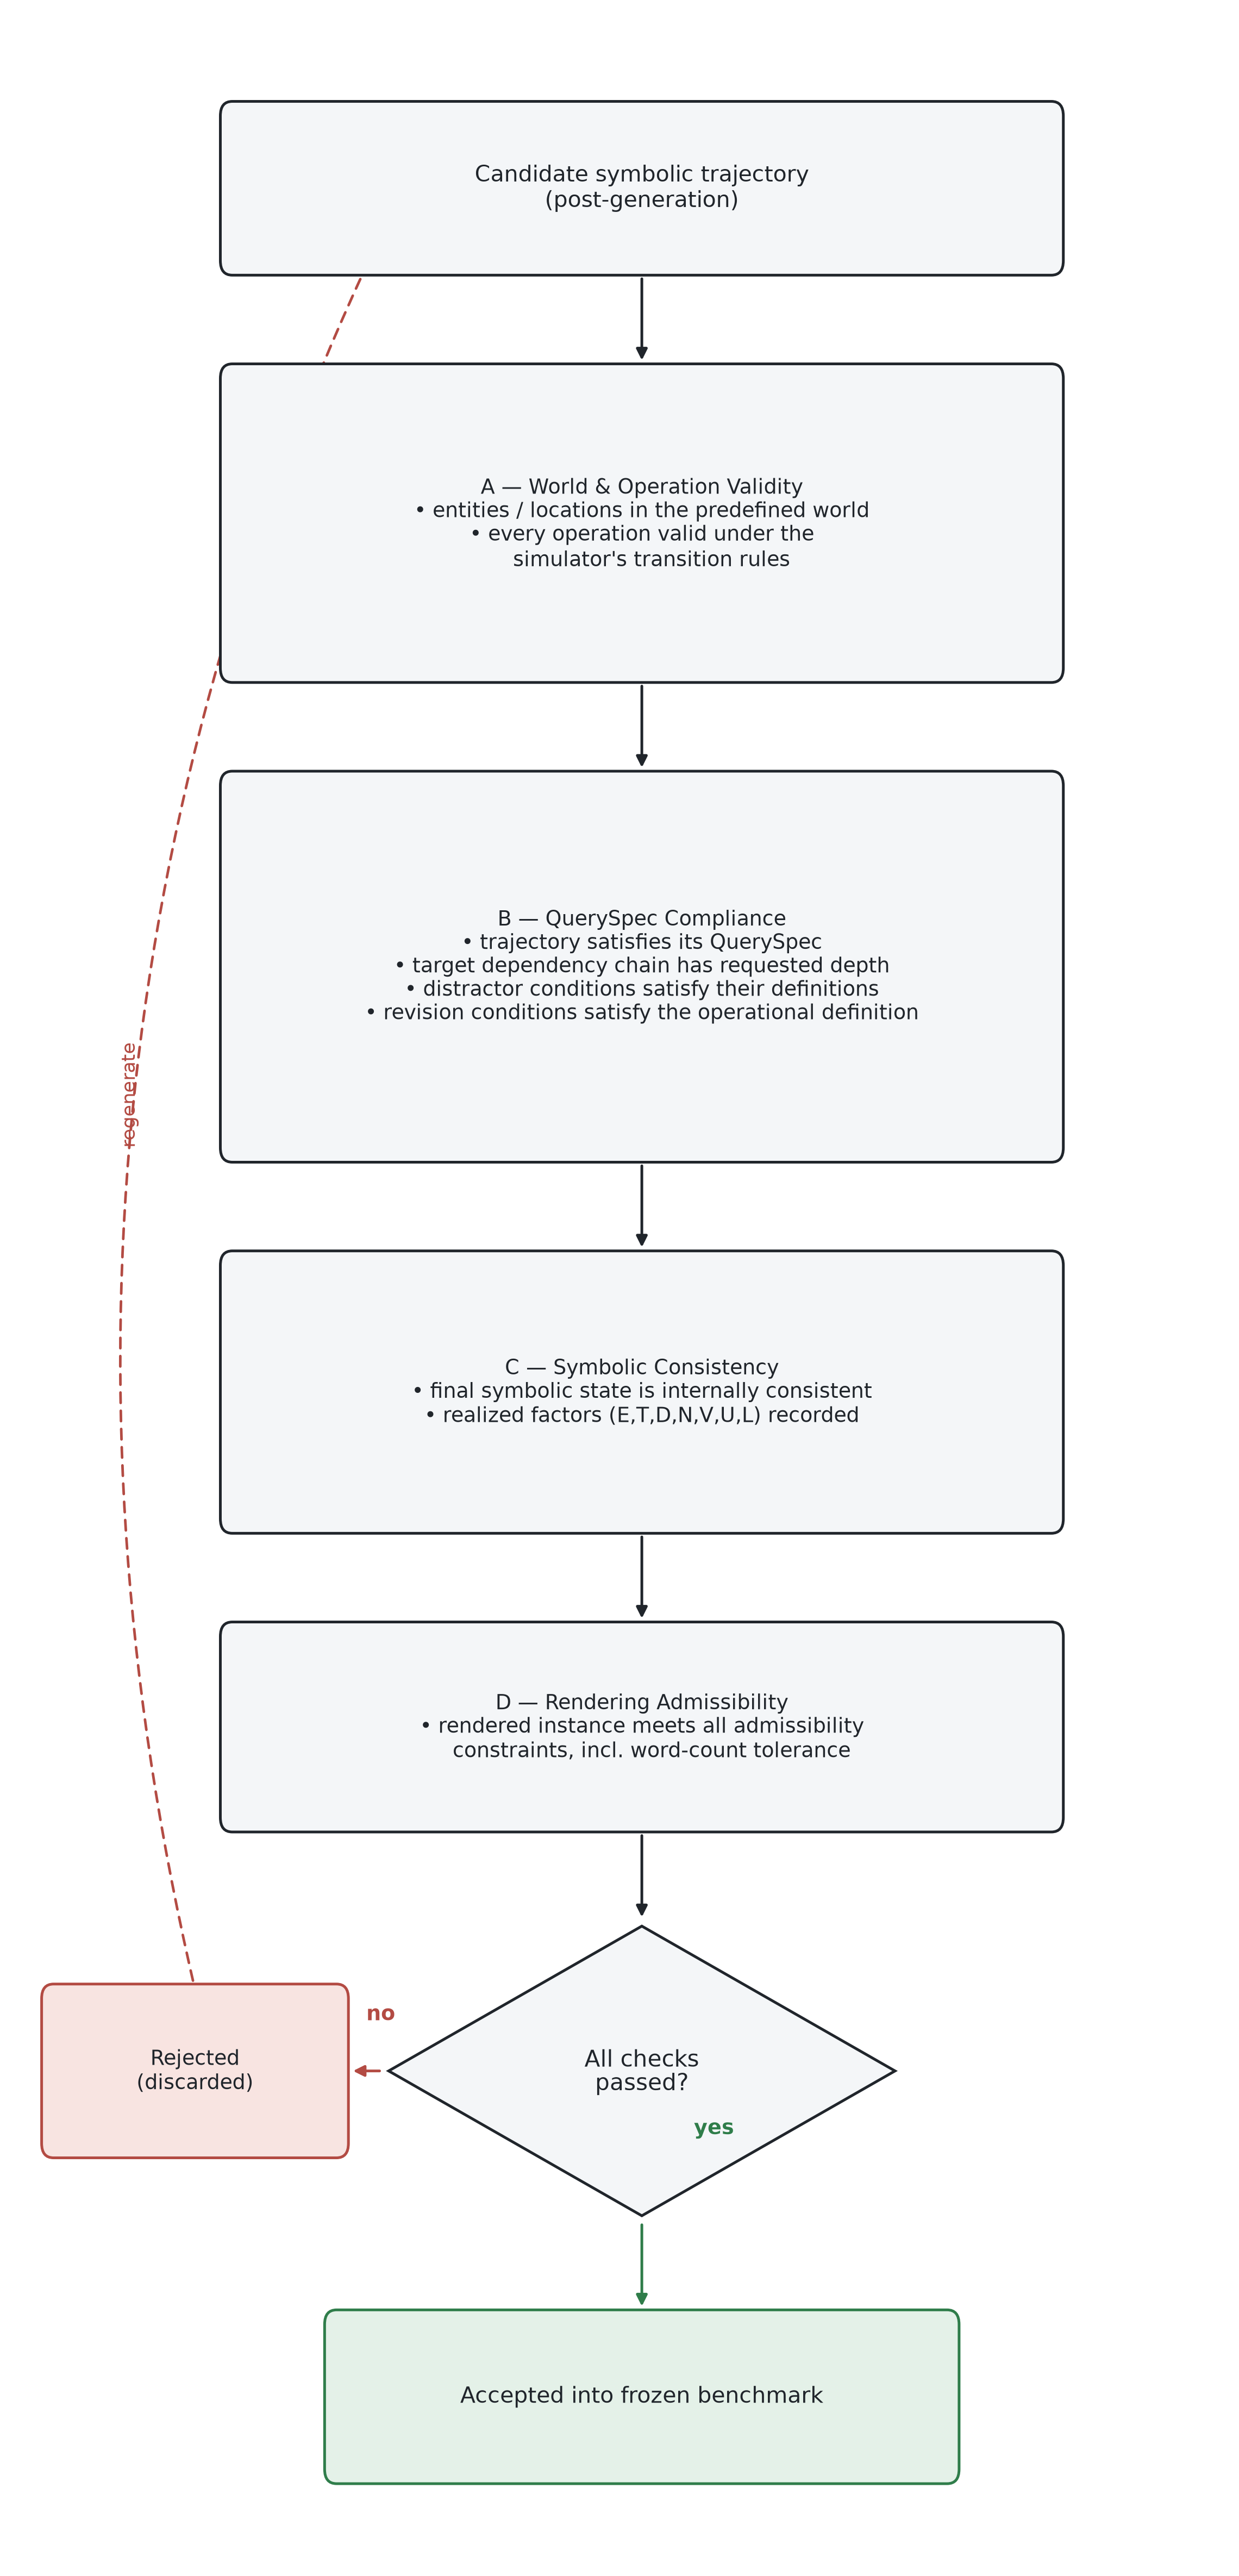
\includegraphics[width=0.55\textwidth]{dws_validation_flow.png}
\caption{Validation flow for DWS-Bench, from structural QuerySpec verification through symbolic
state consistency and rendered-instance admissibility.}
\label{fig:validation-flow}
\end{figure}

\section{Ground-Truth Independence}
The benchmark answer is computed directly from the symbolic simulator:
\[
\mathrm{Answer}=G(S_U,q),
\]
where $S_U$ is the final symbolic world state and $q$ is the query.

The natural-language renderer has no authority over the ground truth. Thus, a rendering error may make
an instance linguistically imperfect, but it cannot silently change the authoritative symbolic label.
This separation is a central requirement of the benchmark's validity.

\chapter{Methodology}
\section{Research Design}
The study is organized into three phases. Phase 1 validates and freezes the benchmark generation
process by measuring realized factor distributions and residual associations. Phase 2 evaluates the
selected Small Language Models on the frozen benchmark and analyzes final-answer accuracy, step-wise
accuracy, performance degradation, and error dynamics. Phase 3 performs a naturalistic reference audit using
procedural narratives to examine whether the controlled findings remain qualitatively relevant outside
the synthetic benchmark.

\section{System Architecture}
The overall workflow separates symbolic trajectory construction from natural-language realization and
model evaluation. The pipeline is:
\[
\text{QuerySpec}
\rightarrow
\text{Generator}
\rightarrow
\text{Validator}
\rightarrow
\text{Renderer}
\rightarrow
\text{SLM}
\rightarrow
\text{Evaluator}.
\]

\begin{figure}[H]
\centering
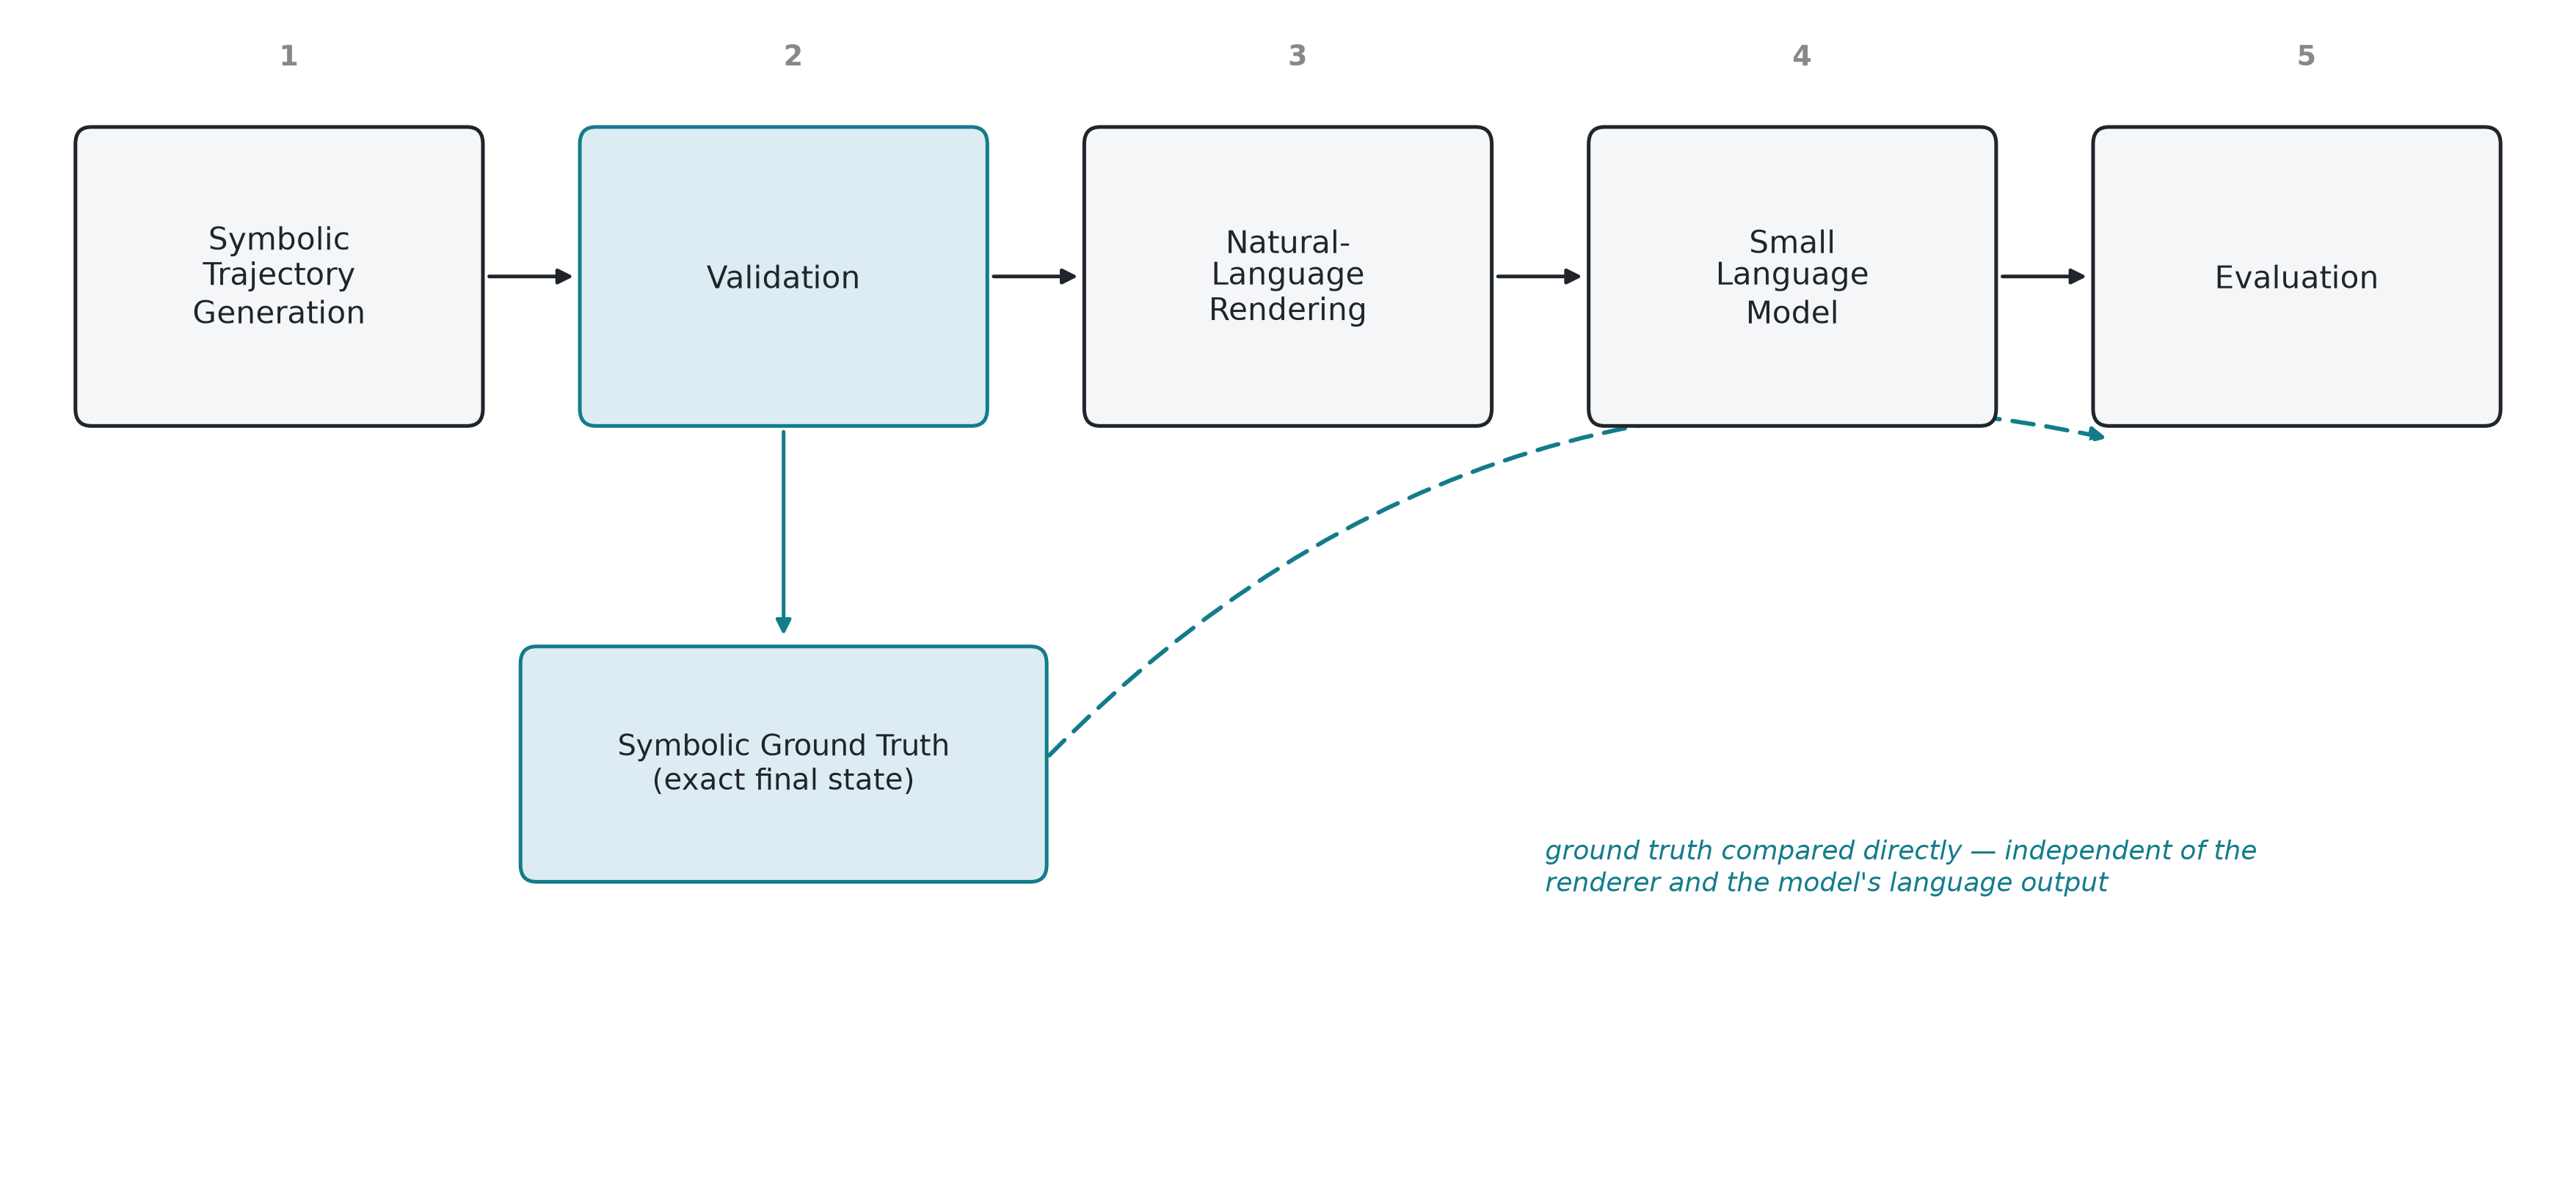
\includegraphics[width=0.95\textwidth]{dws_system_overview.png}
\caption{Overview of the DWS-Bench workflow, separating symbolic trajectory generation, validation,
natural-language rendering, model inference, and evaluation.}
\label{fig:system-overview}
\end{figure}

\begin{figure}[H]
\centering
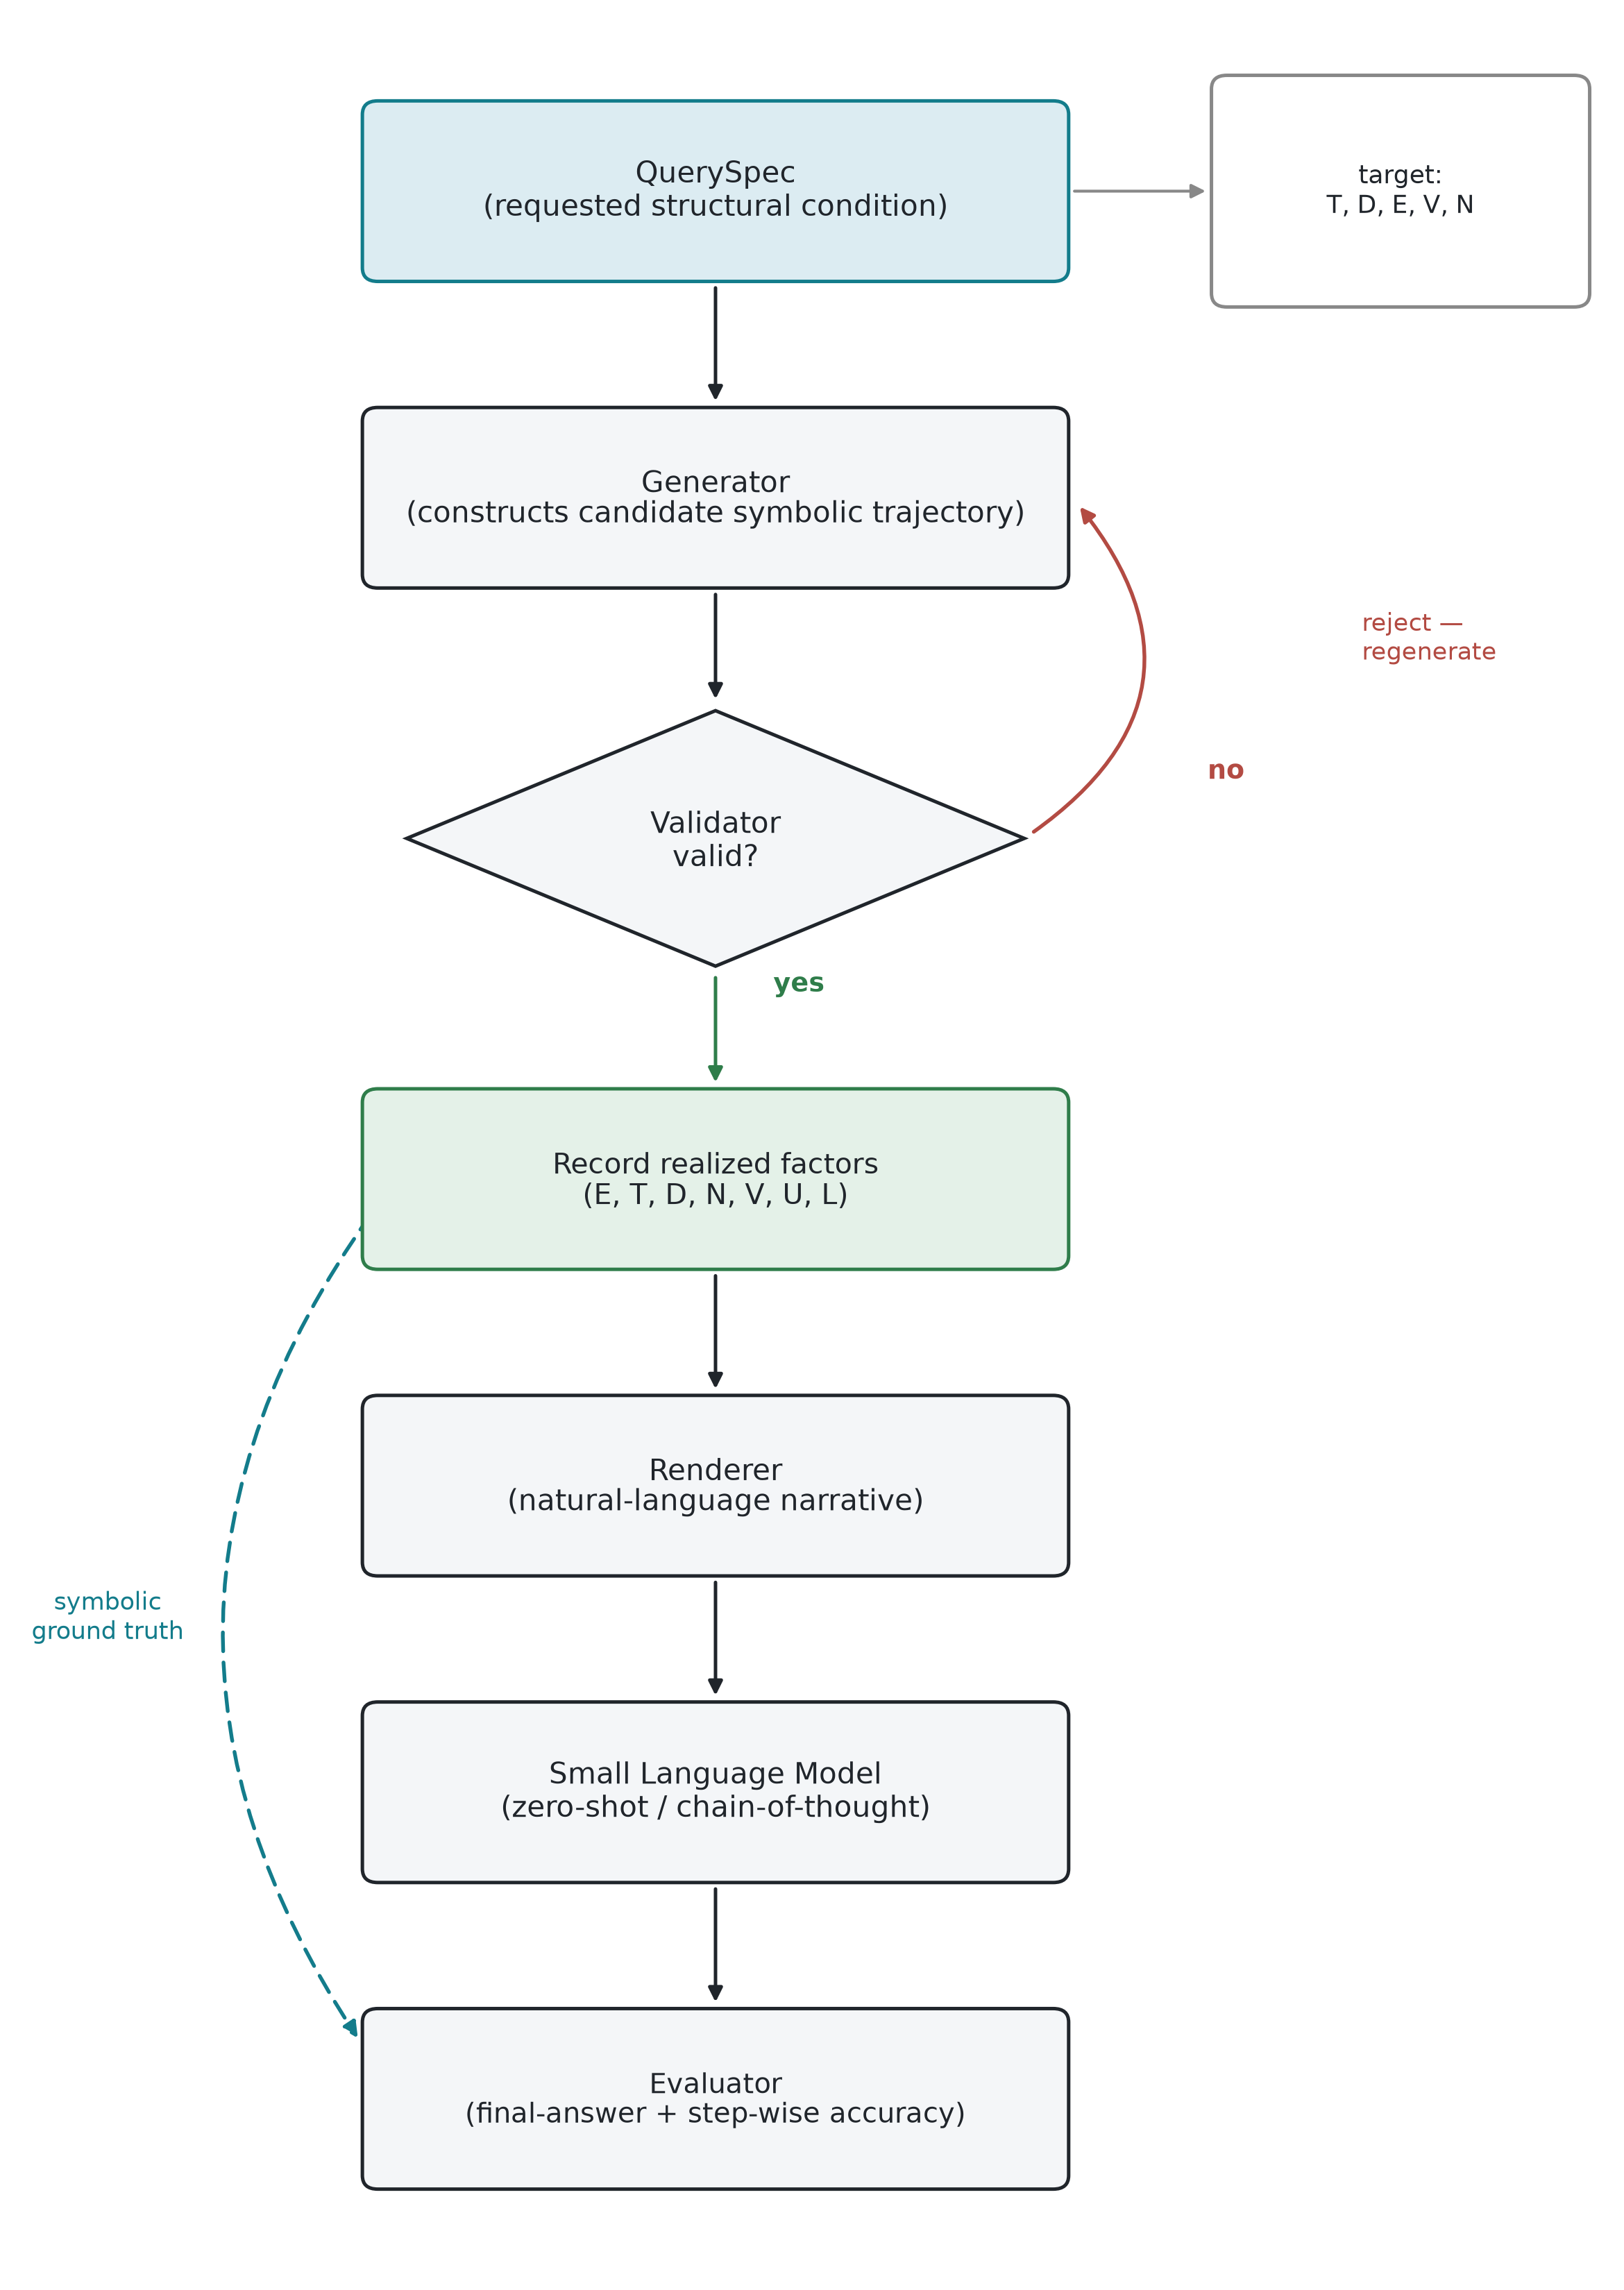
\includegraphics[width=0.7\textwidth]{dws_pipeline_flow.png}
\caption{Detailed DWS-Bench pipeline from structural condition specification to model evaluation.}
\label{fig:pipeline-flow}
\end{figure}

\section{Symbolic World Simulator}
The simulator maintains the authoritative state of every entity and applies all operation semantics
symbolically. State transitions are executed before natural-language rendering, and the resulting
trajectory records the state after each canonical operation.

For a simple movement,
\[
(e_i,l_a)\rightarrow(e_i,l_b).
\]
More complex operations use their corresponding deterministic transition functions. The simulator
therefore provides both the final state used for final-answer evaluation and the intermediate states
used for step-wise evaluation.

\begin{figure}[H]
\centering
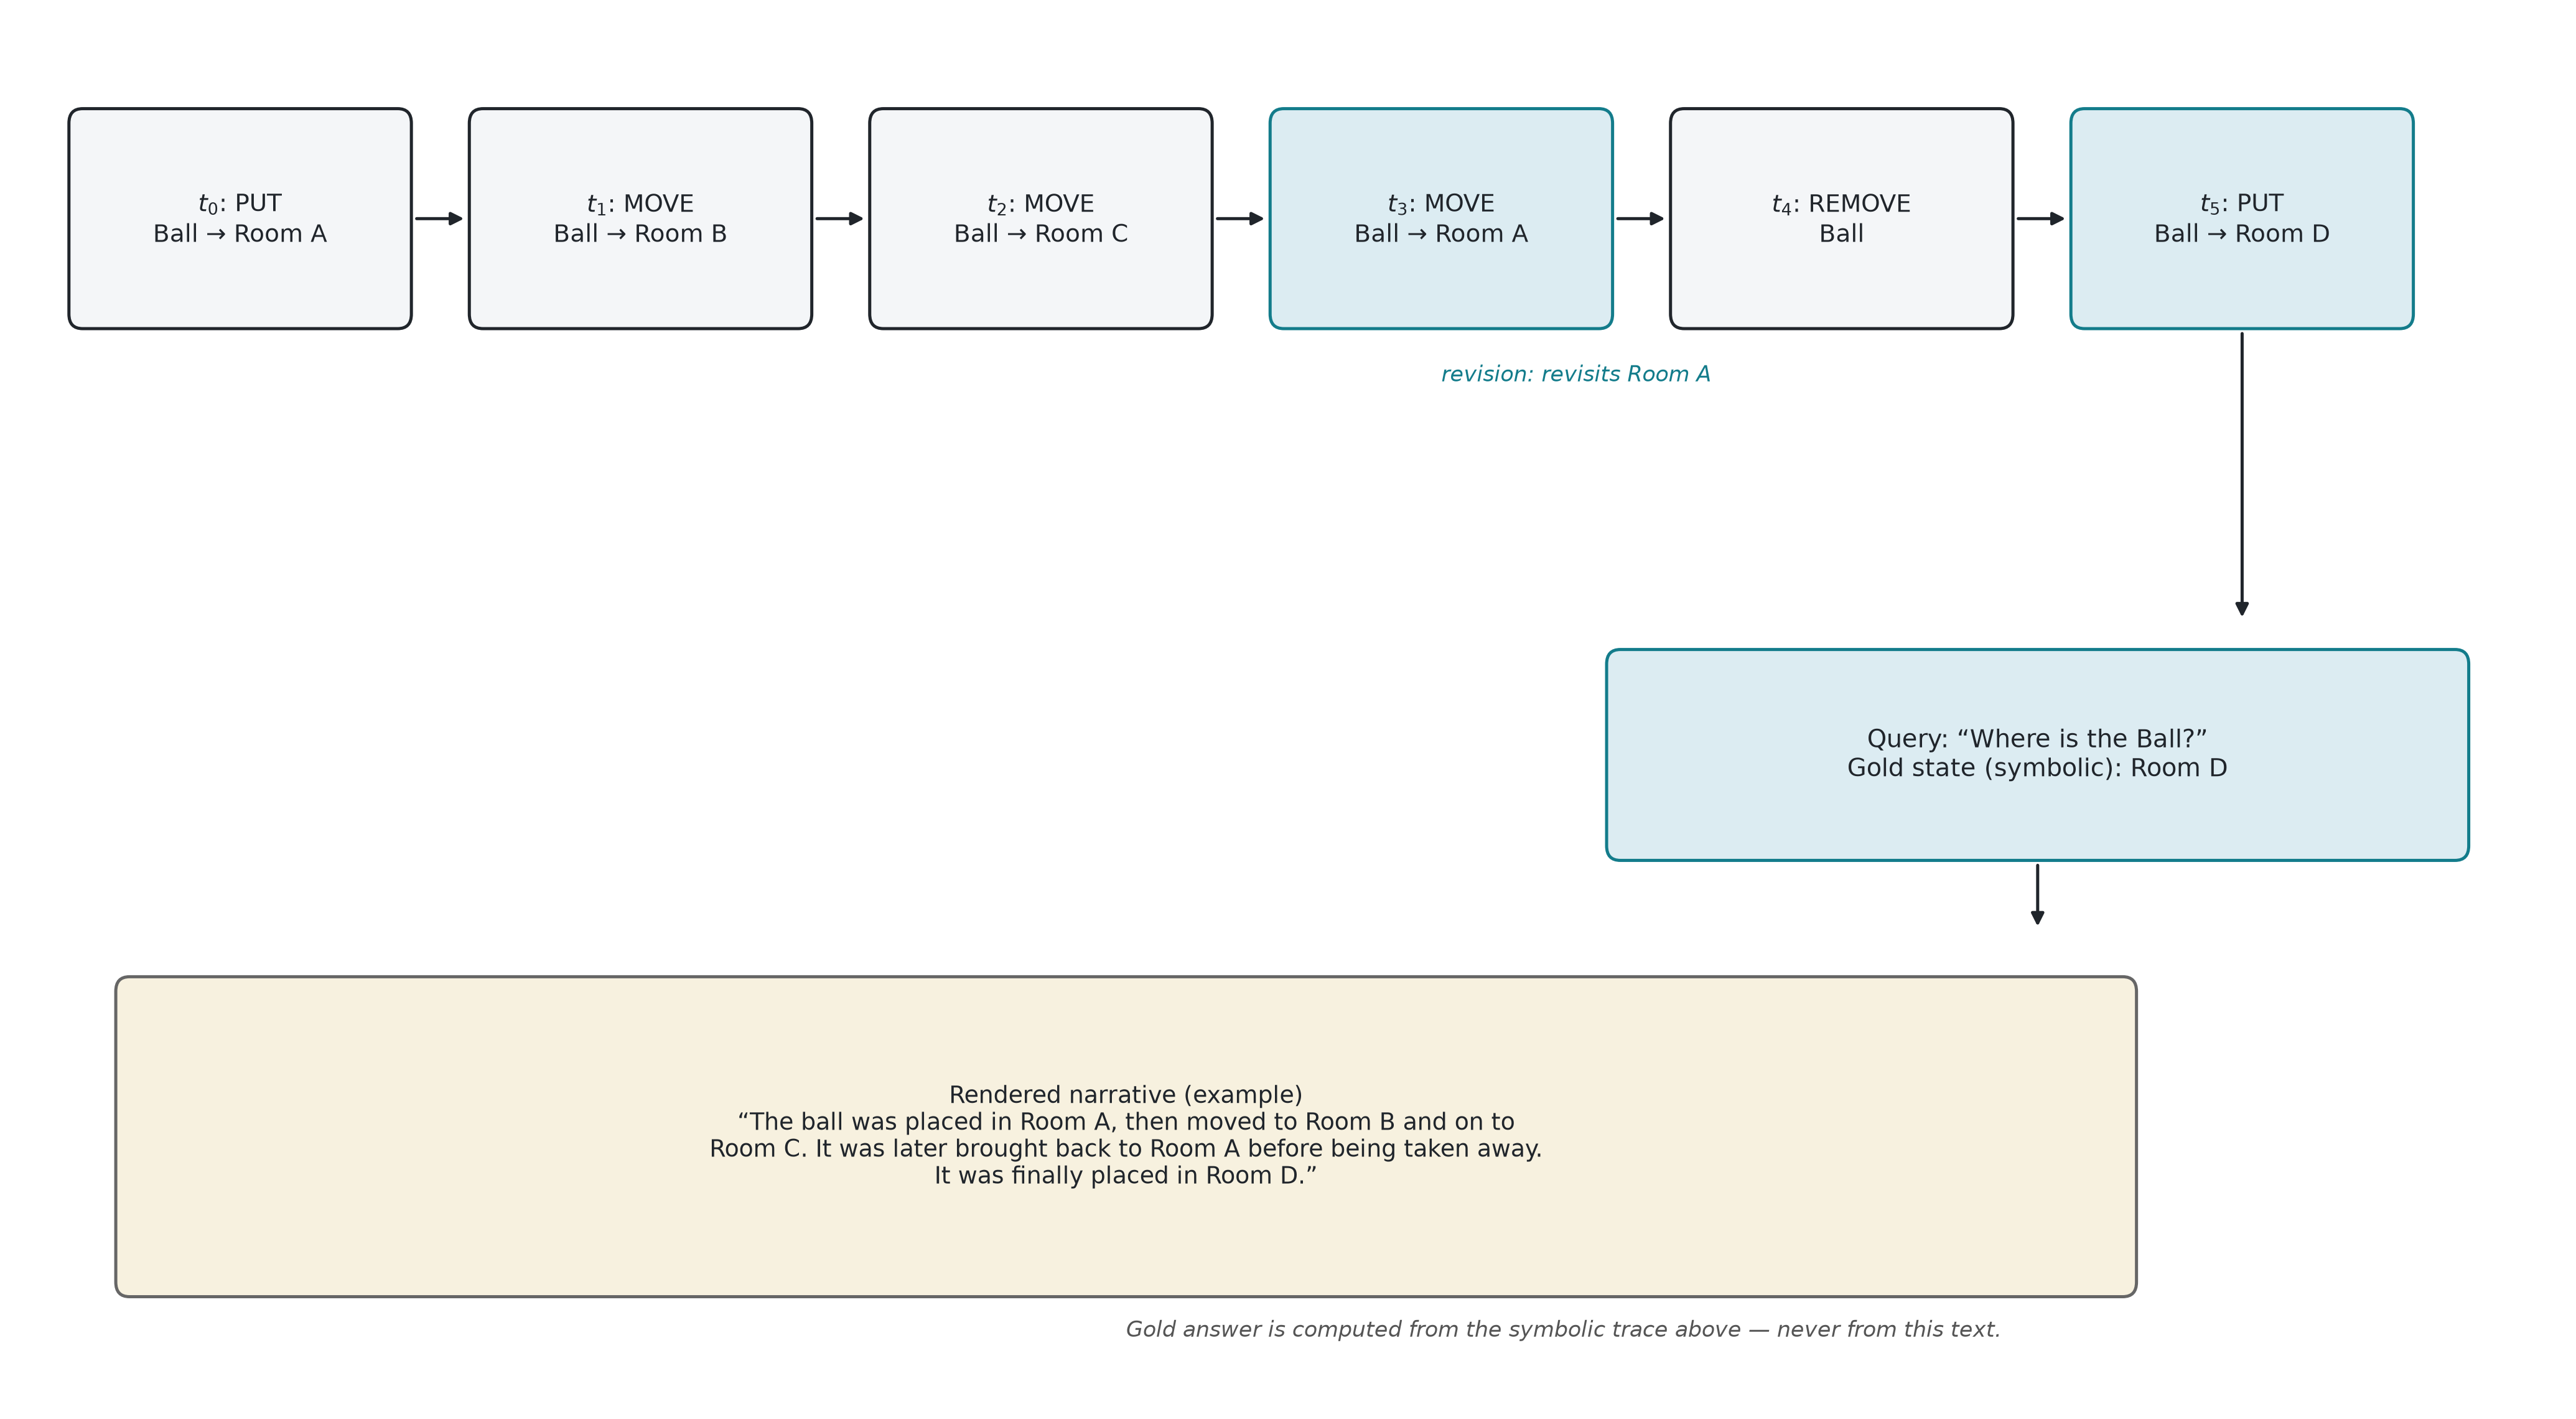
\includegraphics[width=\textwidth]{dws_example_trajectory.png}
\caption{Example symbolic trajectory, revision event, symbolic gold state, and rendered narrative.}
\label{fig:example-trajectory}
\end{figure}

\section{QuerySpec-Driven Generation}
The generator does not rely on unconstrained random trajectories followed by heuristic query selection.
Instead, a QuerySpec describes the structural properties required for a benchmark instance. Candidate
trajectories are generated against these requirements and passed through validation.

This approach separates two responsibilities: the generator creates a valid symbolic trajectory, while
the structural analysis layer determines whether that trajectory and query satisfy the intended
experimental condition. Only validated instances proceed to rendering.

\section{Sampling and Factor Measurement}
Sampling varies surface realizations while preserving the binding structural requirements of the
condition. Entity identities, location identities, operation realizations, and random seeds may vary
without changing the intended factor settings.

For each accepted instance, the implementation records
\[
(E,T,D,N,V,U,L)_{\mathrm{actual}}.
\]
The requested values are therefore not treated as sufficient evidence of experimental control; the
realized values are measured directly from the generated instance.

\begin{figure}[H]
\centering
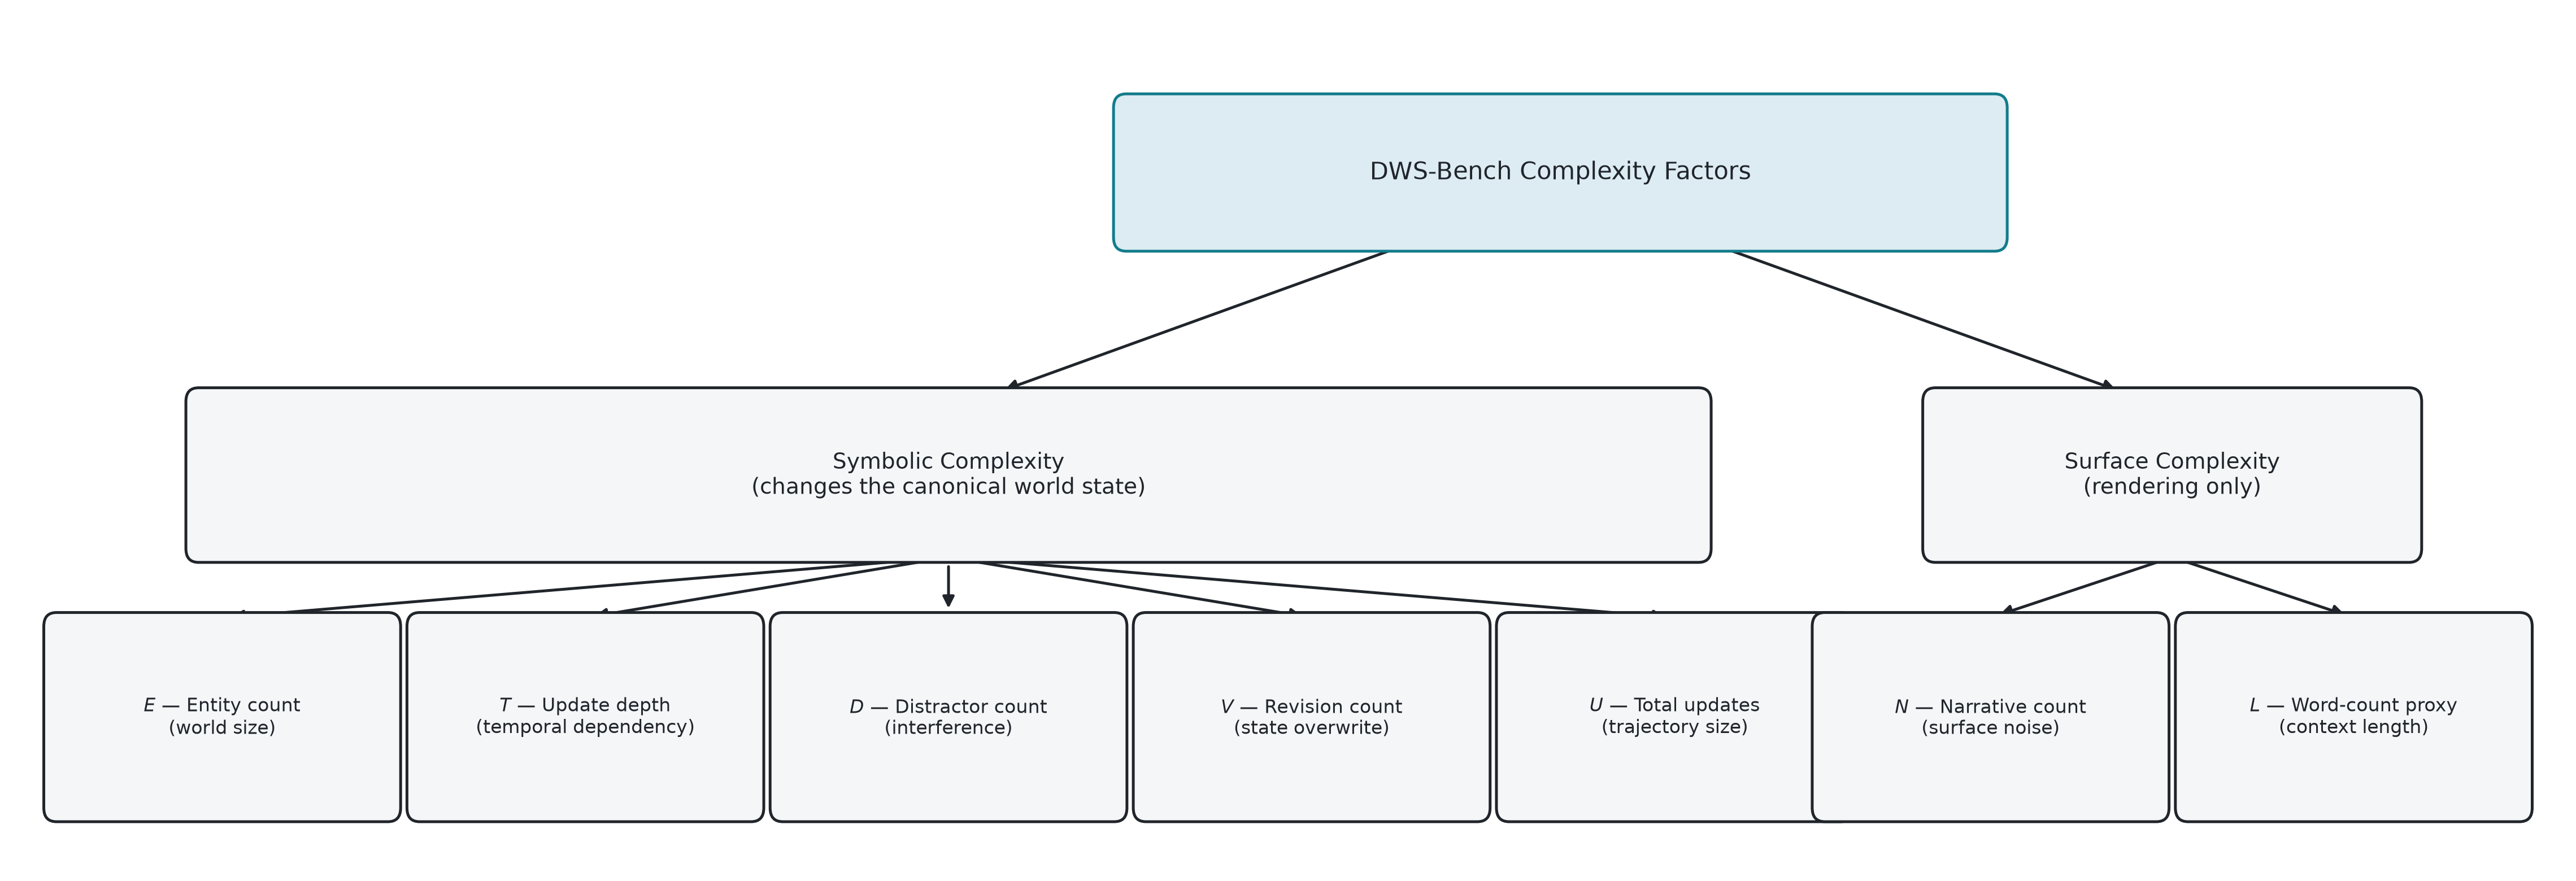
\includegraphics[width=\textwidth]{dws_factor_taxonomy.png}
\caption{DWS-Bench complexity factors separated into symbolic state complexity and rendering-only surface complexity.}
\label{fig:factor-taxonomy}
\end{figure}

\section{Phase 1: Generator Validation}
Phase 1 validates the generator before benchmark datasets are frozen. The analysis examines:
\begin{enumerate}
\item the empirical distribution of each controlled factor;
\item rejection rates at each generation stage;
\item realized word-count distributions;
\item pairwise associations among the measured factors;
\item agreement between requested QuerySpec constraints and realized trajectories.
\end{enumerate}

If a requested condition is not realized reliably, the generator or sampling procedure is revised
before the benchmark is frozen. This prevents model results from being interpreted using nominal
conditions that the generated data do not actually satisfy.

\section{Phase 2: Small Language Model Evaluation}
The model registry defines three core instruction-tuned Small Language Models that were evaluated in the
current study:
\begin{itemize}
\item Qwen2.5-0.5B;
\item Qwen2.5-3B;
\item Qwen2.5-7B.
\end{itemize}

Each model is evaluated in two prompting conditions: a direct zero-shot condition and a
structured chain-of-thought condition in which the model is prompted to reason and answer in a structured way before answering. The two
conditions are reported separately because prior work shows that chain-of-thought changes both the
level and the mechanism of state tracking: it improves entity tracking by decomposing the tracking
demand into shorter contexts over which the model must maintain state signals \cite{tang2026track},
and stronger models benefit disproportionately from it \cite{rezaee2025exploring}.

All models are evaluated using the same frozen benchmark instances and a fixed evaluation protocol.
The protocol records the model identifier, inference configuration, prompt version, decoding settings,
and evaluation seed where applicable. No benchmark condition is modified after observing model
outputs.

\section{Final-Answer and Step-Wise Evaluation}
Final-answer accuracy measures whether the model reports the correct state for the queried entity after
the complete trajectory.

Step-wise accuracy evaluates the model against the canonical symbolic state after each target-relevant
update. Let $\hat{S}_t$ denote the state inferred from the model's response at step $t$ and $S_t$ the
corresponding simulator state. Step-wise accuracy is computed from their agreement under the same
predefined normalization rules used for final answers.

The normalization procedure removes only formatting variation that does not alter the predicted state.
It must not transform an incorrect state into a correct one or permit semantically different answers to
match.

\section{RQ1: Temporal Depth}
RQ1 varies target-relevant update depth while keeping the intended non-depth conditions fixed. The
analysis plots accuracy as a function of $T$ and identifies the region in which performance changes
from stable to substantially degraded.

Because increasing $T$ also lengthens the rendered narrative, RQ1 includes a length-only control
condition. In this control, $T$ is held at a low value while narrative distractors are added to
reproduce the rendered-length distribution of the higher-depth conditions. Comparing the depth
conditions against this control separates the effect of additional state updates from the effect of
a longer context.

The analysis is not limited to a single aggregate score. Step-wise trajectories are used to determine
whether errors emerge gradually or after a particular dependency depth.

\section{RQ2: State Revision}
RQ2 tests whether models correctly overwrite previously valid state information. A revision is counted
only when the trajectory deliberately revisits or reverses a previously established state relationship
according to the benchmark's revision specification. Revision is therefore a structural property of
the trajectory, not merely a count of MOVE operations.

The revision experiment compares matched control and revision conditions so that the effect of revision
can be distinguished from the general difficulty of the trajectory.

\section{RQ3: Distractor Interference}
RQ3 evaluates interference from information unrelated to the queried entity. State-changing distractor
updates and narrative-level distractors are treated as distinct factors. The state-changing sweep
varies $D$ while holding the target chain fixed; a matched condition adds $N=4$ state-neutral sentences
to the $D=4$ condition. The $D$ and $N$ conditions are constructed at matched rendered length, so the
comparison separates symbolic interference from surface-level noise rather than from a difference in
context length. The analysis reports the two mechanisms separately.

\section{RQ4: Entity Load}
RQ4 evaluates entity load using a dedicated interleaved-chain sweep with $E\in\{2,3,4,5\}$,
$T=8$, and $D=4$. The target receives the same requested number of updates in every condition while
the pool of distractor entities changes. Realized word length is reported as a possible residual
confound. Stable queried-entity accuracy across entity-load conditions is treated as a meaningful
empirical outcome rather than as evidence that the experiment failed.

\section{RQ5: Structural Operation Pilot}
RQ5 is a pilot across the \texttt{split\_chain}, \texttt{merge\_chain}, \texttt{swap\_chain},
\texttt{undo\_chain}, and \texttt{undo\_redo\_chain} families at a requested depth of $T=8$. Its purpose is to verify generation and
evaluation coverage for the broader operation algebra. Realized factors must be reported: the
\texttt{split\_chain} records realize $T_{\mathrm{actual}}=7$ and $D_{\mathrm{actual}}=1$, while the
available records for the other four pilot families realize $T_{\mathrm{actual}}=8$ in the frozen data.
The pilot should therefore not be described as a perfectly matched depth comparison.

\section{Counterfactual Probe Support}
The repository contains support for constructing counterfactual probes by changing a controlled
operation or state transition while preserving the surrounding context as closely as the generator
permits. No populated counterfactual probe results are included in the current evaluation artifacts,
so this capability is treated as infrastructure for future experiments rather than as an empirical
finding in this thesis.

\section{Phase 3: Naturalistic Reference Audit Status}
The naturalistic reference set has been prepared as a secondary analysis resource, but no model-level
results are included in the current evaluation artifacts. Accordingly, this phase is exploratory and
does not contribute an empirical claim to the main conclusions. Because the naturalistic setting would
introduce uncontrolled linguistic and semantic variation, it would not support the same causal claims
as the controlled experiments.

\chapter{Implementation}
\section{Implementation Architecture}
The repository is organized around the following modules:
\begin{table}[H]
\centering
\begin{tabular}{ll}
\toprule
\textbf{Module} & \textbf{Responsibility} \\
\midrule
Contract / QuerySpec & Experimental condition and structural specification \\
Simulator & Symbolic world-state transitions and canonical states \\
Generator & Controlled trajectory construction \\
Validator & Structural, semantic, and admissibility verification \\
Sampler & Instance sampling and surface variation \\
Renderer & Natural-language realization \\
Evaluator & Model inference and metric computation \\
Analysis & Factor distributions, performance degradation, and error dynamics \\
Tests & Unit, smoke, and robustness testing \\
\bottomrule
\end{tabular}
\caption{DWS-Bench implementation architecture.}
\label{tab:implementation}
\end{table}

\section{Operation Implementation}
The simulator implements eight operation types:
PUT, MOVE, REMOVE, UNDO, REDO, SPLIT, MERGE, and SWAP. Each operation is represented symbolically
before rendering. This allows the validator to inspect the state transition directly and permits the
evaluator to obtain canonical intermediate states for step-wise scoring.

\begin{figure}[H]
\centering
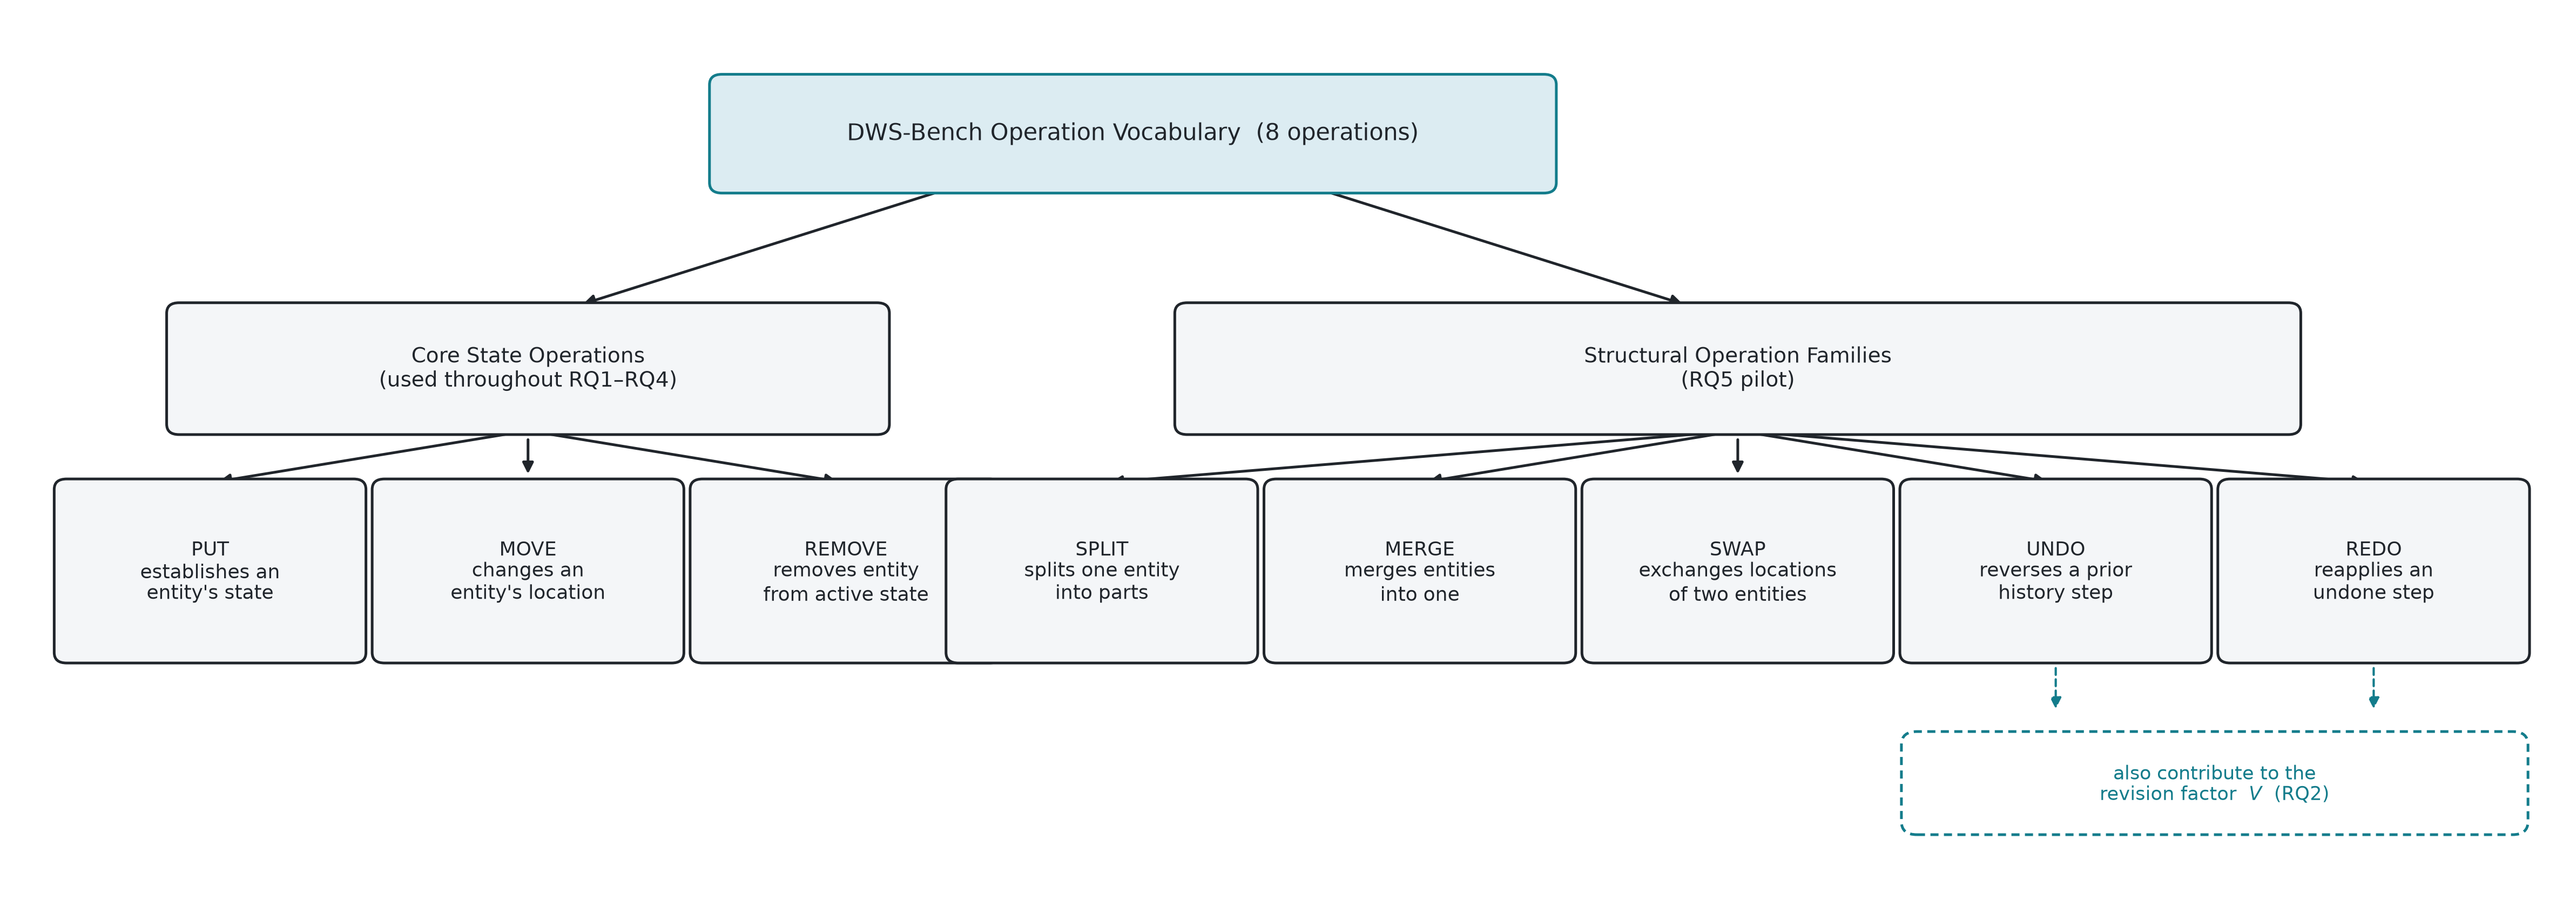
\includegraphics[width=\textwidth]{dws_operation_taxonomy.png}
\caption{DWS-Bench operation vocabulary, separating core state operations from structural operation families.}
\label{fig:operation-taxonomy}
\end{figure}

\section{Implementation Status}
The implementation status at the time of writing is summarized below. The benchmark and the model-level
results reported in this thesis are based on the completed evaluation artifacts currently available in
the repository. RQ4 remains unevaluated at the model-output level, while RQ5 has been evaluated as a
structural-operation pilot within the core benchmark.
\begin{table}[H]
\centering
\begin{tabular}{lll}
\toprule
\textbf{Component} & \textbf{Status} & \textbf{Evidence} \\
\midrule
Symbolic simulator & Completed & Unit/smoke tests \\
Eight-operation vocabulary & Completed & Operation tests \\
QuerySpec layer & Completed & Specification tests \\
Trajectory generator & Completed & Generator tests \\
Experimental contract & Completed & Contract tests \\
Validator & Completed & Validation tests \\
Sampler & Completed & Sampling tests \\
Renderer & Completed & Rendering examples \\
Evaluation harness & Completed & Evaluation pipeline \\
Phase 1 validation & Completed & Factor-distribution analysis \\
Phase 2 SLM evaluation & Completed & 3x2 model-prompt configs on all instances \\
Phase 3 naturalistic audit & Pilot / descriptive & Procedural reference set \\
\bottomrule
\end{tabular}
\caption{Implementation status at the time of writing.}
\label{tab:implementation-status}
\end{table}

\section{Reproducibility}
Each experiment records the random seed where applicable, benchmark version, QuerySpec, generator
version, requested and realized factor values, valid and rejected instance counts, word-count
statistics, model identifier, inference configuration, and evaluation configuration. This metadata
supports reproduction of both the benchmark and the subsequent model evaluation.

\chapter{Results and Discussion}
\label{chap:results}
\section{Results Reporting Protocol}
The results are organized around the five research questions and the three study phases. Phase 1 reports
whether the generator realizes the intended benchmark conditions. Phase 2 reports model performance and
failure behavior on the frozen benchmark, including the structural-operation families in RQ5. Phase 3
records the status of the naturalistic reference audit.

The repository contains the frozen benchmark and the implementation-verification artifacts. The model
results reported here were obtained from the repository's stored evaluation summaries for three
Qwen2.5 parameter-scale variants under both chain-of-thought and non-chain-of-thought prompting, all evaluated on the
same 1,150-instance evaluation set.

\section{Phase 1: Generator Validation}
Phase 1 validates the benchmark at the level of realized structural factors before interpreting model
performance. The generator is designed to preserve the intended experimental contracts in the frozen
benchmark and to record the realized values of $(E,T,D,N,V,U,L)$ rather than assuming that nominally
requested conditions remain exact in the rendered narrative.

\begin{table}[H]
\centering
\begin{tabular}{p{0.12\textwidth}p{0.17\textwidth}p{0.22\textwidth}p{0.37\textwidth}}
\toprule
\textbf{Factor} & \textbf{Requested} & \textbf{Realized} & \textbf{Status} \\
\midrule
$E$ & $1$--$5$ & $1$--$5$ & Verified across the frozen benchmark \\
$T$ & $2$--$16$ & $2$--$16$ & Realized in the depth sweep \\
$D$ & $0$--$16$ & $0$--$16$ & Realized in the distractor sweep \\
$N$ & $\{0,4\}$ & $\{0,4\}$ & Matched in the narrative-distractor condition \\
$V$ & Requested by slice & $0$--$14$ & Revision is realized through target-state revisits and history-based rewrites \\
$U$ & Total canonical updates & Derived from canonical trace & Recorded as realized update count \\
$L$ & $<600$ words & 32--312 words & Word-count proxy, not tokenizer tokens \\
\bottomrule
\end{tabular}
\caption{Generator-validation summary from the frozen benchmark.}
\label{tab:factor-validation}
\end{table}

The factor measurements matter because they support interpretation of model degradation as a function of
realized complexity rather than nominal specification alone. In particular, the validation step confirms
that the benchmark contains hard cases with sustained temporal dependencies, state revisits, and
irrelevant state changes without allowing these conditions to be conflated with mere narrative length.

\section{Phase 2: Model Evaluation}
The benchmark was evaluated with the three Qwen2.5 parameter-scale variants represented in the repository results, under
both chain-of-thought and non-chain-of-thought prompting. The full configuration-level comparison is
reported below.

\begin{table}[H]
\centering
\resizebox{\textwidth}{!}{%
\begin{tabular}{lcccc}
\toprule
\textbf{Model} & \textbf{Prompting} & \textbf{Final Accuracy} & \textbf{Step-wise Accuracy} & \textbf{Instances} \\
\midrule
Qwen2.5-0.5B & No CoT & 40.87\% & 25.39\% & 1150 \\
Qwen2.5-0.5B & CoT & 0.17\% & -- & 1150 \\
Qwen2.5-3B & No CoT & 25.65\% & 24.07\% & 1150 \\
Qwen2.5-3B & CoT & 49.91\% & 2.82\% & 1150 \\
Qwen2.5-7B & No CoT & 11.39\% & -- & 1150 \\
Qwen2.5-7B & CoT & 10.52\% & 23.99\% & 1150 \\
\bottomrule
\end{tabular}
}%
\caption{Overall benchmark performance across the evaluated model families and prompting conditions.}
\label{tab:model-summary}
\end{table}

\begin{figure}[H]
\centering
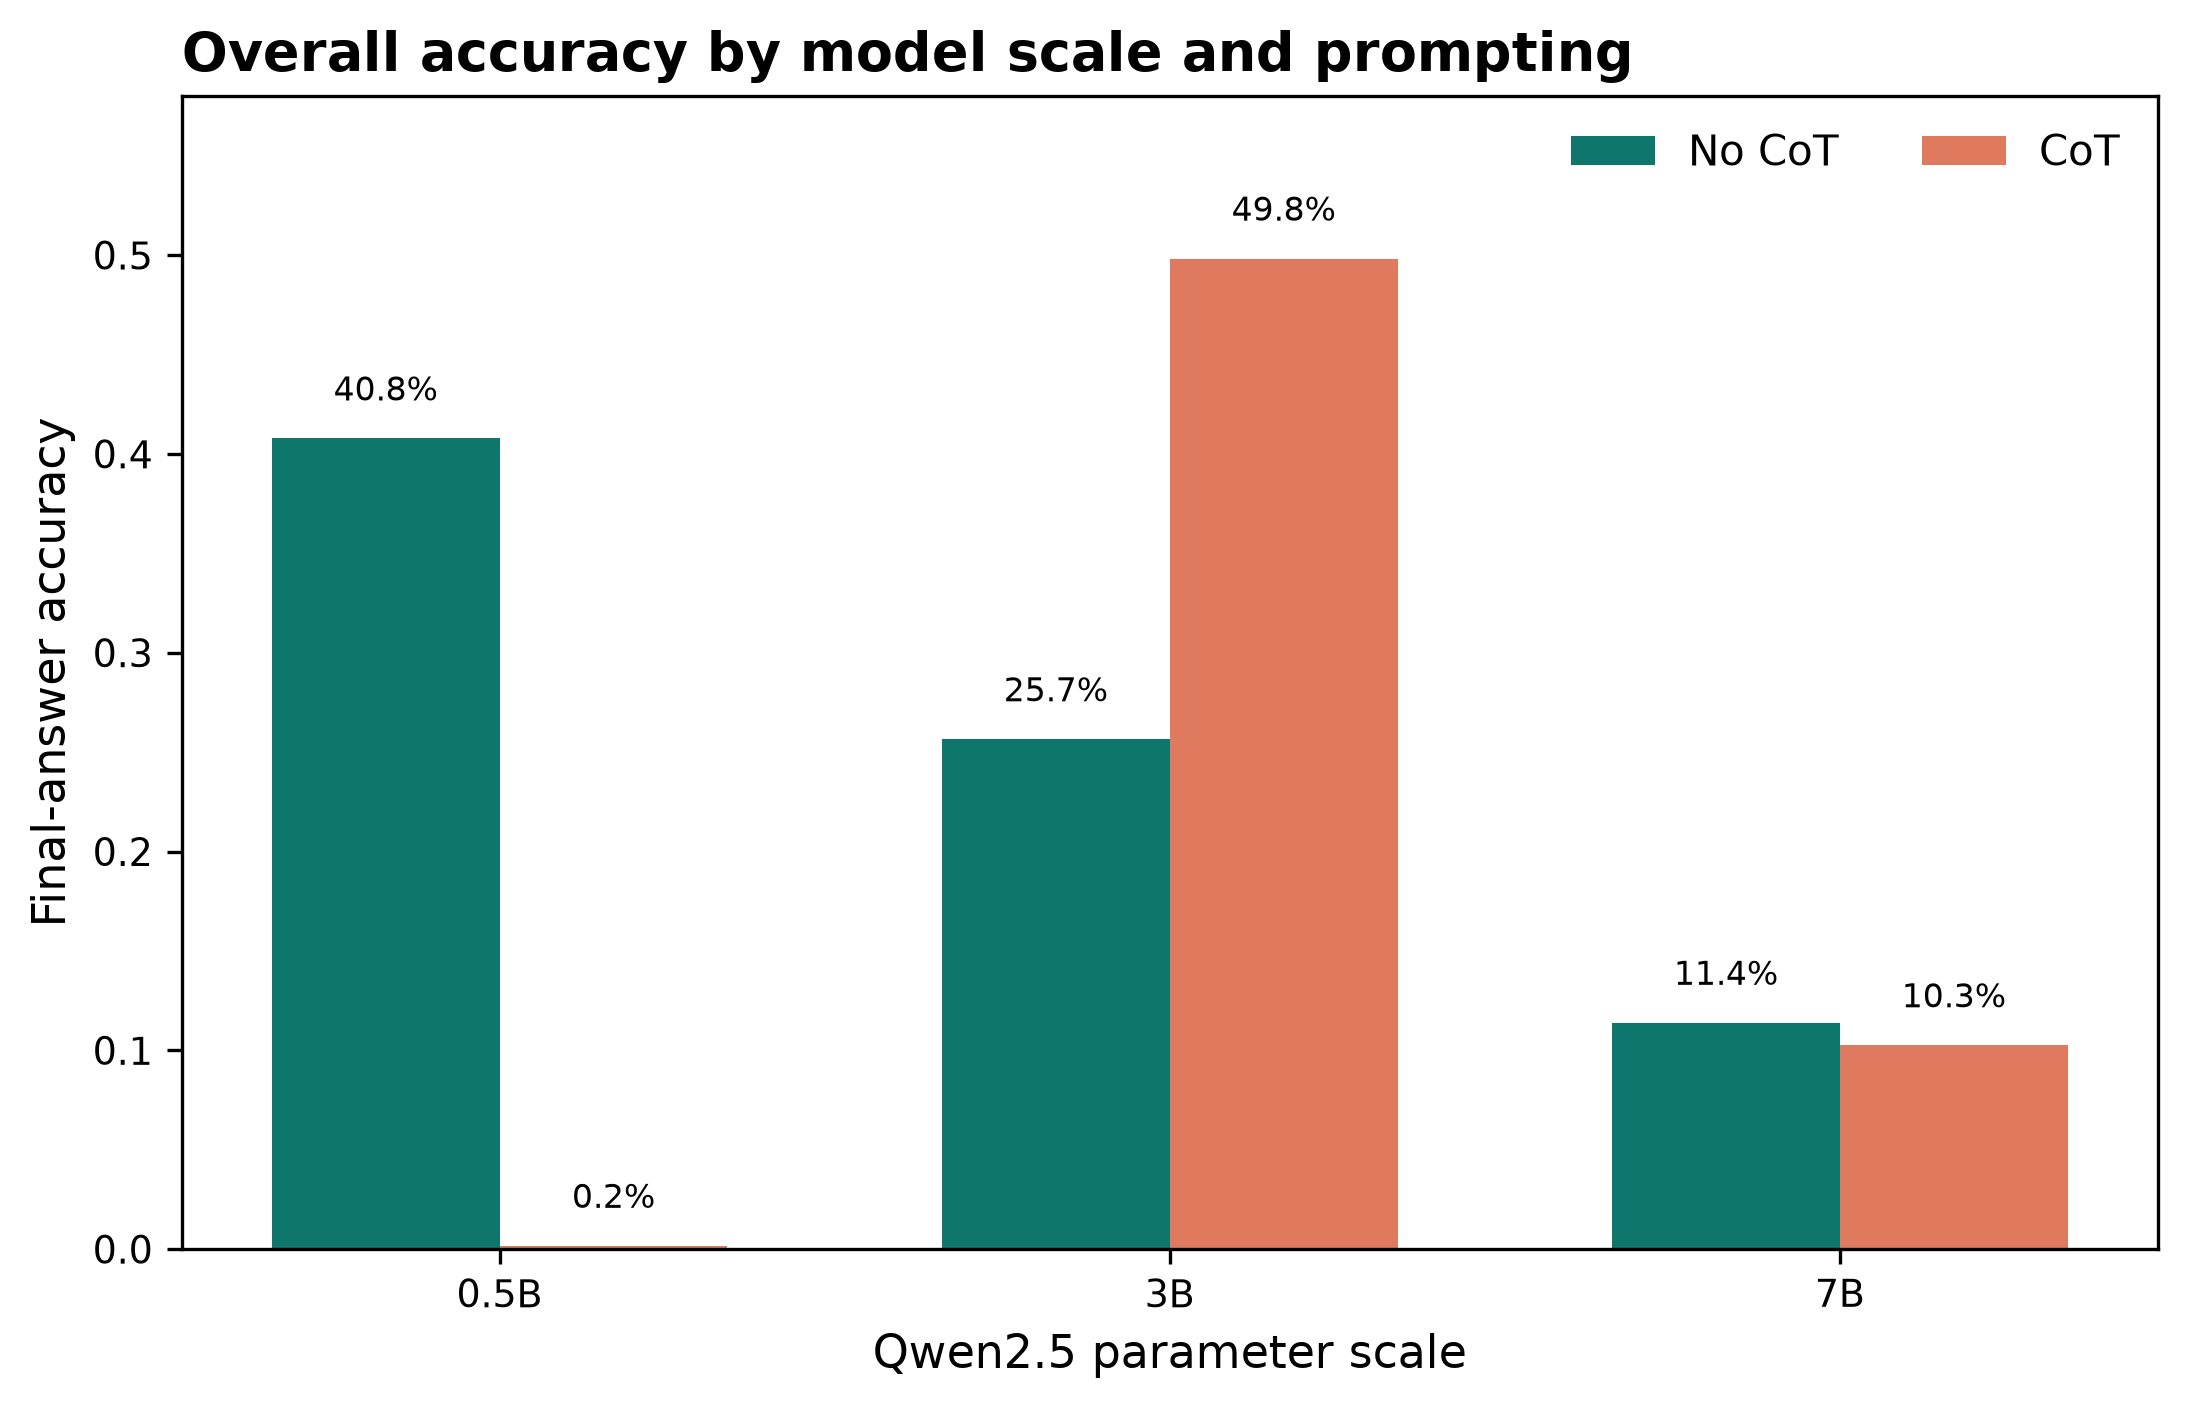
\includegraphics[width=\textwidth]{fig01_overall_model_prompting.png}
\caption{Overall final-answer accuracy across model scales and prompting conditions.}
\label{fig:overall-model-prompting}
\end{figure}

Among all six model-prompt configurations, the strongest overall result was achieved by Qwen2.5-3B with
chain-of-thought prompting, reaching 49.91\% final-answer accuracy. Qwen2.5-0.5B without CoT was the
next strongest configuration at 40.87\%, while the CoT variant of the same 0.5B model collapsed to
0.17\%. The 3B non-CoT setting also underperformed relative to the CoT variant at 25.65\%, and the 7B
models remained weak across both prompting regimes. These findings show that the effect of prompting is
highly model-dependent and that the benchmark does not support a simple monotonic relationship between
model scale and reasoning quality.

\section{RQ1 Results: Temporal Depth}
RQ1 examines how final-answer accuracy changes as the target-relevant update depth $T$ increases.
The recorded depth sweep shows a clear contrast between the small model and the stronger 3B model.

\begin{table}[H]
\centering
\resizebox{\textwidth}{!}{%
\begin{tabular}{lcccccc}
\toprule
\textbf{Model} & \textbf{$T=2$} & \textbf{$T=4$} & \textbf{$T=6$} & \textbf{$T=8$} & \textbf{$T=12$} & \textbf{$T=16$} \\
\midrule
Qwen2.5-0.5B (No CoT) & 100.0\% & 66.0\% & 24.0\% & 22.0\% & 46.0\% & 36.0\% \\
Qwen2.5-0.5B (CoT) & 0.0\% & 0.0\% & 0.0\% & 0.0\% & 0.0\% & 0.0\% \\
Qwen2.5-3B (No CoT) & 85.0\% & 88.0\% & 84.0\% & 88.0\% & 84.0\% & 78.0\% \\
Qwen2.5-3B (CoT) & 100.0\% & 100.0\% & 100.0\% & 98.0\% & 98.0\% & 90.0\% \\
Qwen2.5-7B (No CoT) & 6.0\% & 8.0\% & 14.0\% & 10.0\% & 12.0\% & 8.0\% \\
Qwen2.5-7B (CoT) & 10.0\% & 12.0\% & 10.0\% & 16.0\% & 8.0\% & 6.0\% \\
\bottomrule
\end{tabular}
}%
\caption{Final-answer accuracy by target-relevant update depth for the RQ1 sweep across all model and prompting conditions.}
\label{tab:rq1-results}
\end{table}

\begin{figure}[H]
\centering
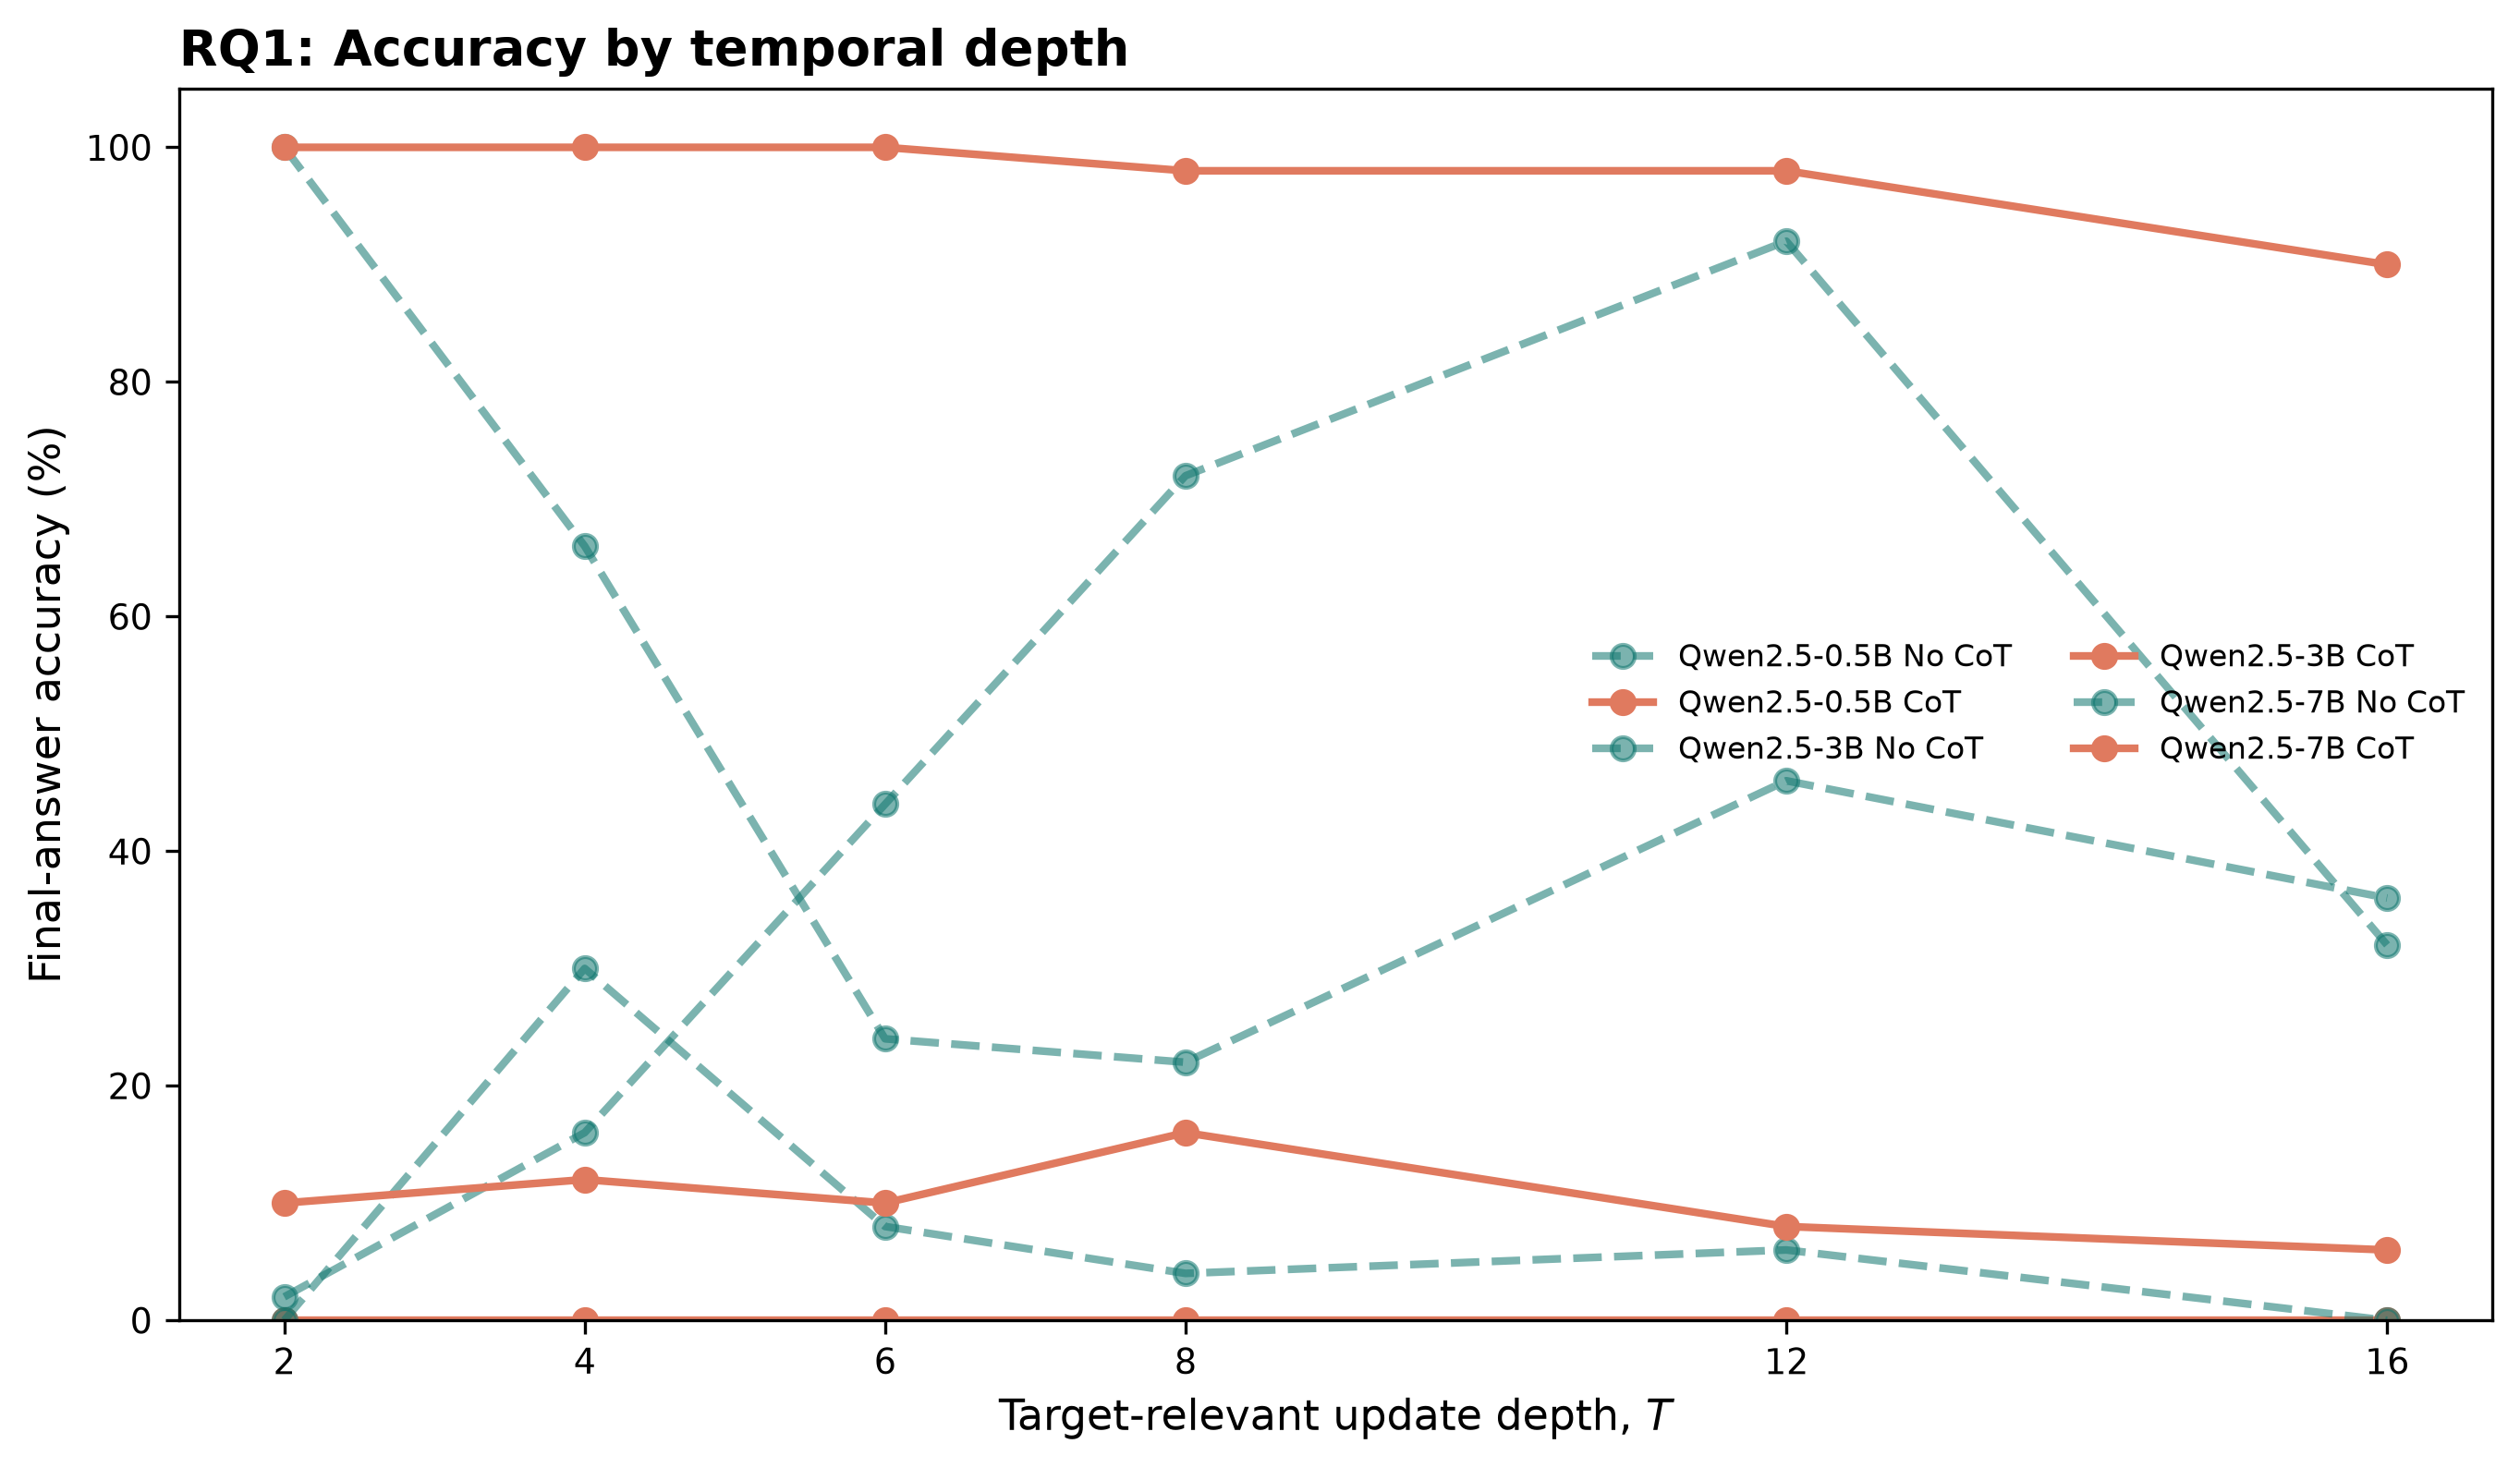
\includegraphics[width=\textwidth]{fig02_rq1_temporal_depth.png}
\caption{RQ1 final-answer accuracy as target-relevant update depth increases.}
\label{fig:rq1-temporal-depth}
\end{figure}

The temporal-depth sweep shows a pronounced difference between the clean baseline and the more demanding
state-tracking conditions. The 0.5B model without CoT shows early degradation between $T=2$ and $T=6$,
with accuracy falling from 100\% to 24\%. The subsequent non-monotonic recovery at $T=12$ indicates that
this degradation is not a single irreversible threshold. The 3B model with CoT remains high-performing
through $T=12$ before declining at $T=16$. The CoT variant of the 0.5B model performed at or near zero
across the depth sweep, indicating that prompt-induced reasoning was not beneficial for this model in this
setting. The 7B models remained weak across all depths regardless of prompting, suggesting that scale
alone did not yield the expected stability in dynamic state retention.

\section{RQ2 Results: State Revision}
RQ2 evaluates how repeated revisits to prior state information affect reasoning accuracy under matched
state depth. The revision family is stronger than the clean depth sweep because it forces the model to
recover the current location after the state has been overwritten or revisited multiple times.

\begin{table}[H]
\centering
\begin{tabular}{lcccc}
\toprule
\textbf{Model} & \textbf{$T=4$} & \textbf{$T=8$} & \textbf{$T=12$} & \textbf{$T=16$} \\
\midrule
Qwen2.5-0.5B (No CoT) & 48.0\% & 40.0\% & 40.0\% & 30.0\% \\
Qwen2.5-0.5B (CoT) & 0.0\% & 0.0\% & 0.0\% & 0.0\% \\
Qwen2.5-3B (No CoT) & 6.0\% & 10.0\% & 8.0\% & 4.0\% \\
Qwen2.5-3B (CoT) & 6.0\% & 76.0\% & 2.0\% & 2.0\% \\
Qwen2.5-7B (No CoT) & 4.0\% & 0.0\% & 4.0\% & 0.0\% \\
Qwen2.5-7B (CoT) & 4.0\% & 14.0\% & 0.0\% & 0.0\% \\
\bottomrule
\end{tabular}
\caption{Final-answer accuracy on the revision sweep for RQ2 across all model and prompting conditions.}
\label{tab:rq2-results}
\end{table}

\begin{figure}[H]
\centering
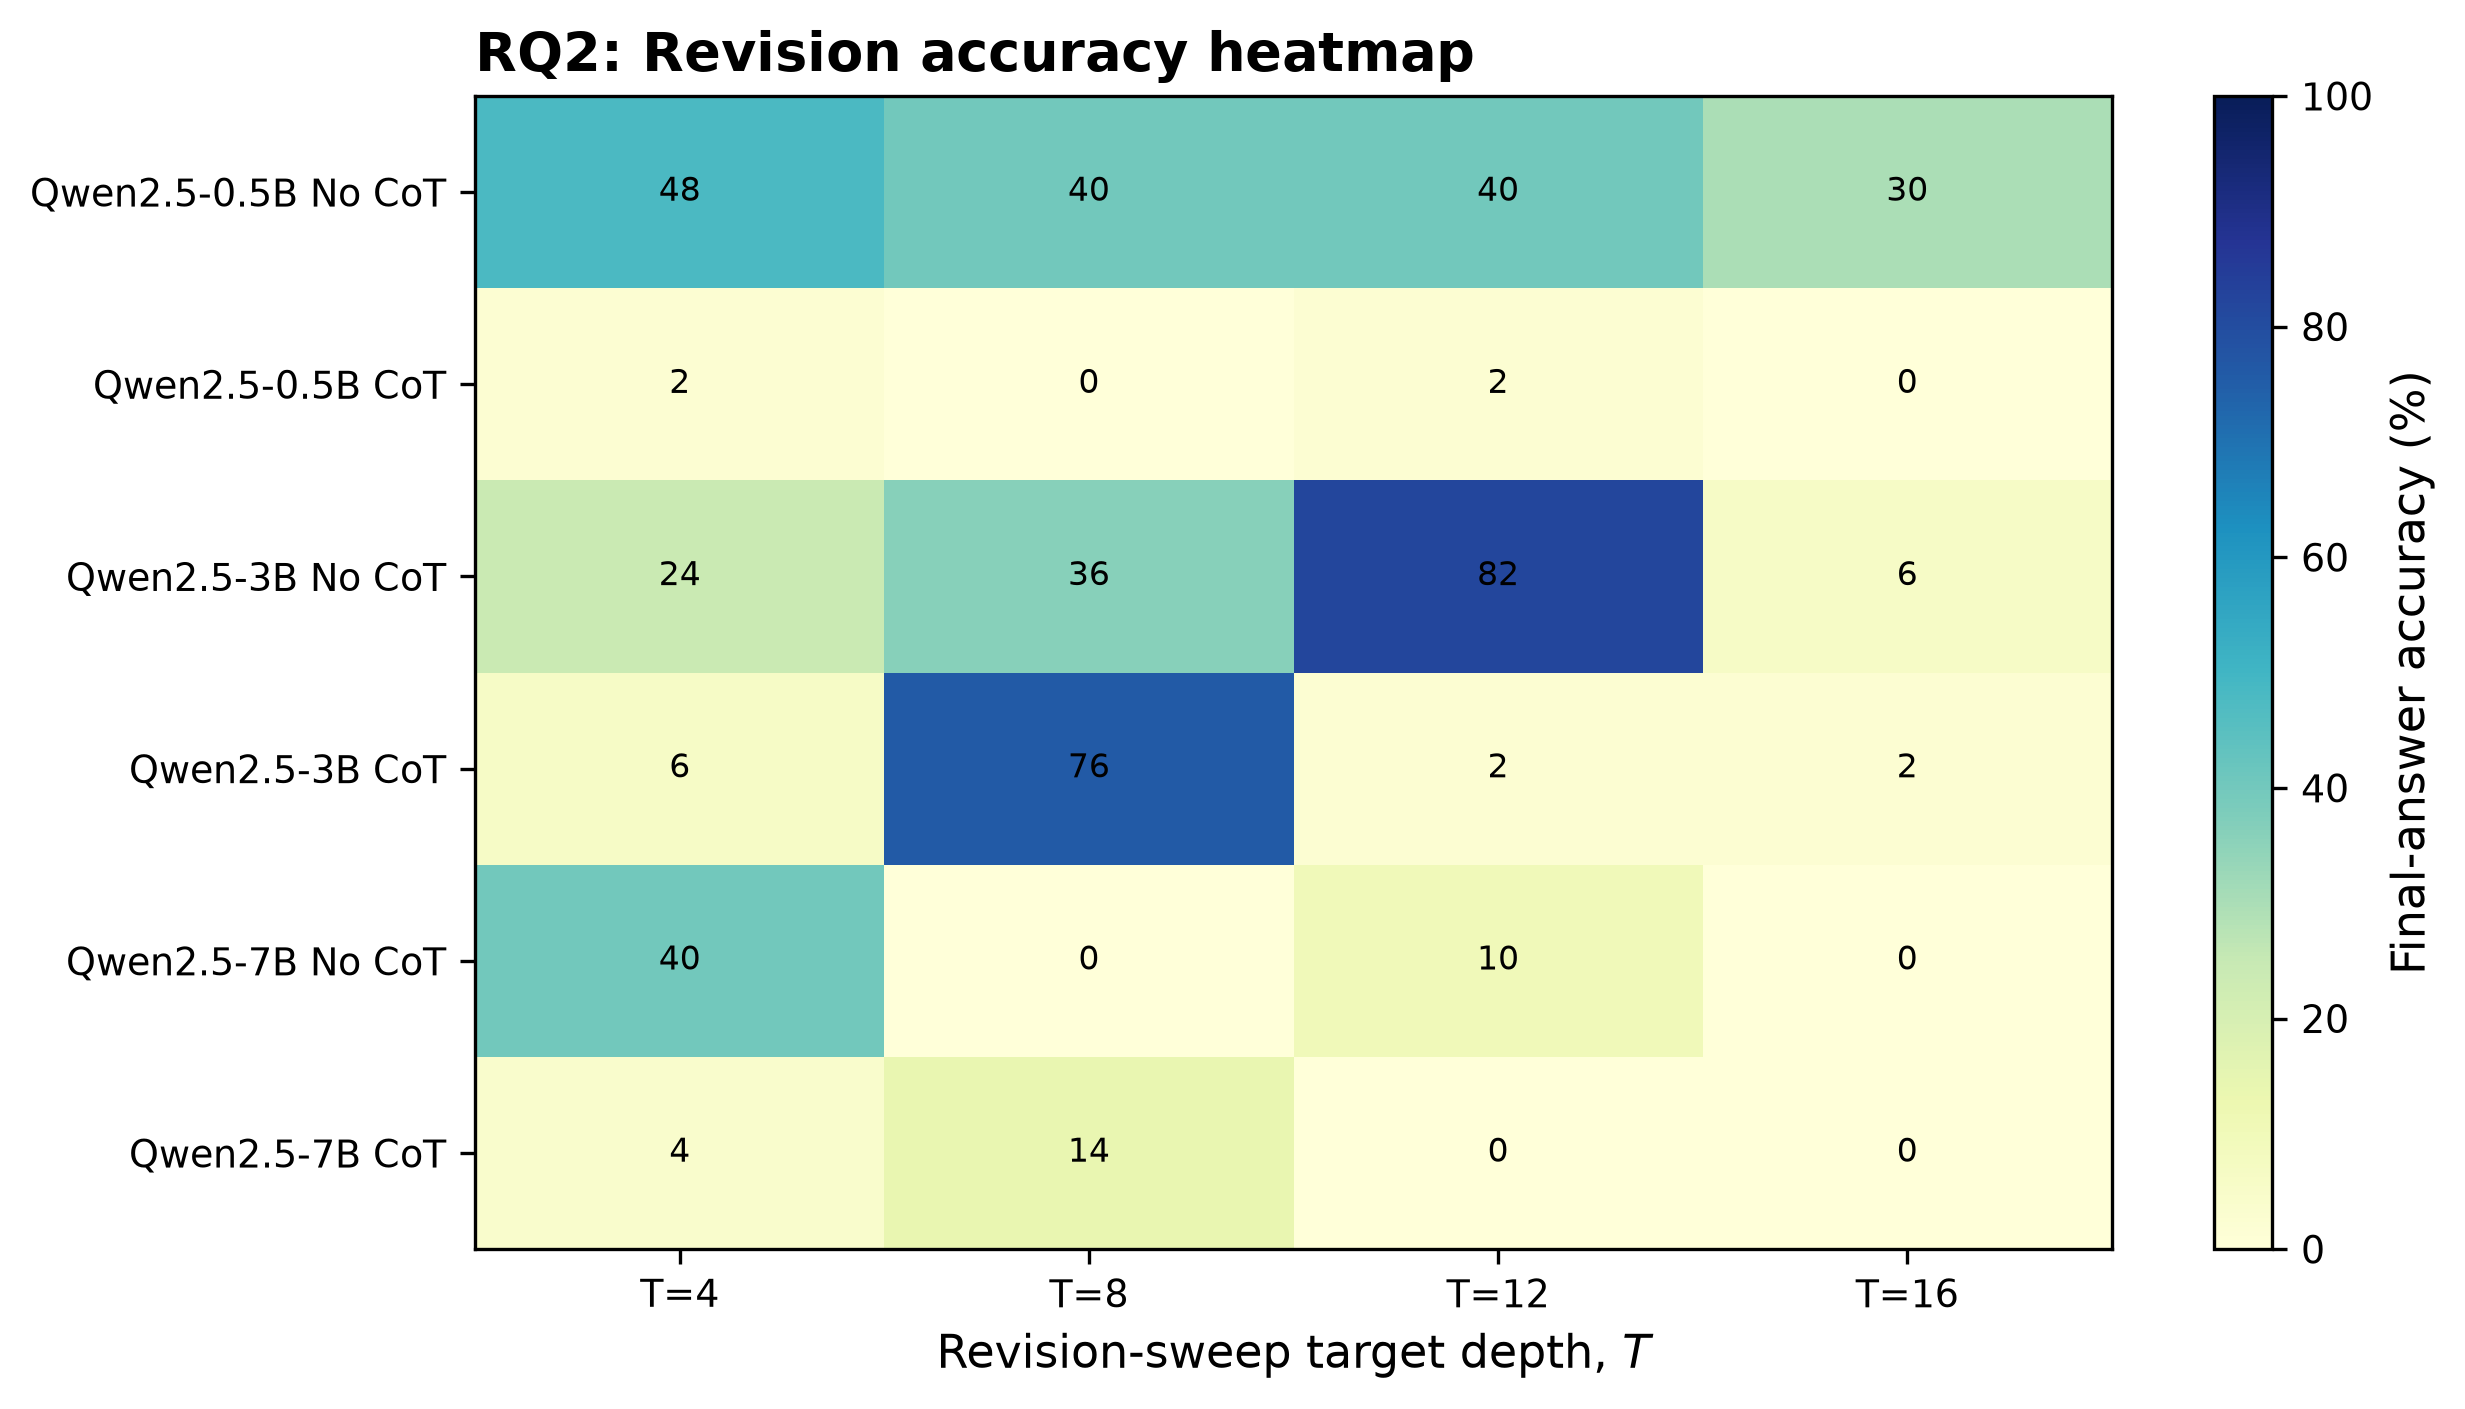
\includegraphics[width=\textwidth]{fig03_rq2_revision_heatmap.png}
\caption{RQ2 final-answer accuracy across revision depth and model-prompting configurations.}
\label{fig:rq2-revision-heatmap}
\end{figure}

These results indicate that state revision is a substantial source of failure under the evaluated
conditions. The 0.5B model without CoT declines from 48\% at $T=4$ to 30\% at $T=16$, while the 3B
model with CoT performs erratically, reaching 76\% at $T=8$ but collapsing to 2\%--6\% at the remaining
revision depths. The CoT variant of 0.5B and the 7B models remain weak across the revision conditions,
which indicates that the benchmark is challenging not only for small models but also for models that
attempt explicit reasoning when the state history must be revisited and overwritten.

\section{RQ3 Results: Distractor Interference}
RQ3 examines the effect of state-changing distractors on a fixed target dependency chain. In this sweep,
relevant target updates remain constant while additional irrelevant updates are introduced into the same
trajectory.

\begin{table}[H]
\centering
\begin{tabular}{lccc}
\toprule
\textbf{Model} & \textbf{$D=4$} & \textbf{$D=8$} & \textbf{$D=16$} \\
\midrule
Qwen2.5-0.5B (No CoT) & 29.0\% & 38.0\% & 10.0\% \\
Qwen2.5-0.5B (CoT) & 0.0\% & 0.0\% & 0.0\% \\
Qwen2.5-3B (No CoT) & 18.0\% & 16.0\% & 16.0\% \\
Qwen2.5-3B (CoT) & 18.7\% & 16.0\% & 16.0\% \\
Qwen2.5-7B (No CoT) & 0.0\% & 0.0\% & 0.0\% \\
Qwen2.5-7B (CoT) & 7.0\% & 36.0\% & 52.0\% \\
\bottomrule
\end{tabular}
\caption{Final-answer accuracy under increasing state-changing distractor count for RQ3 across all model and prompting conditions.}
\label{tab:rq3-results}
\end{table}

\begin{figure}[H]
\centering
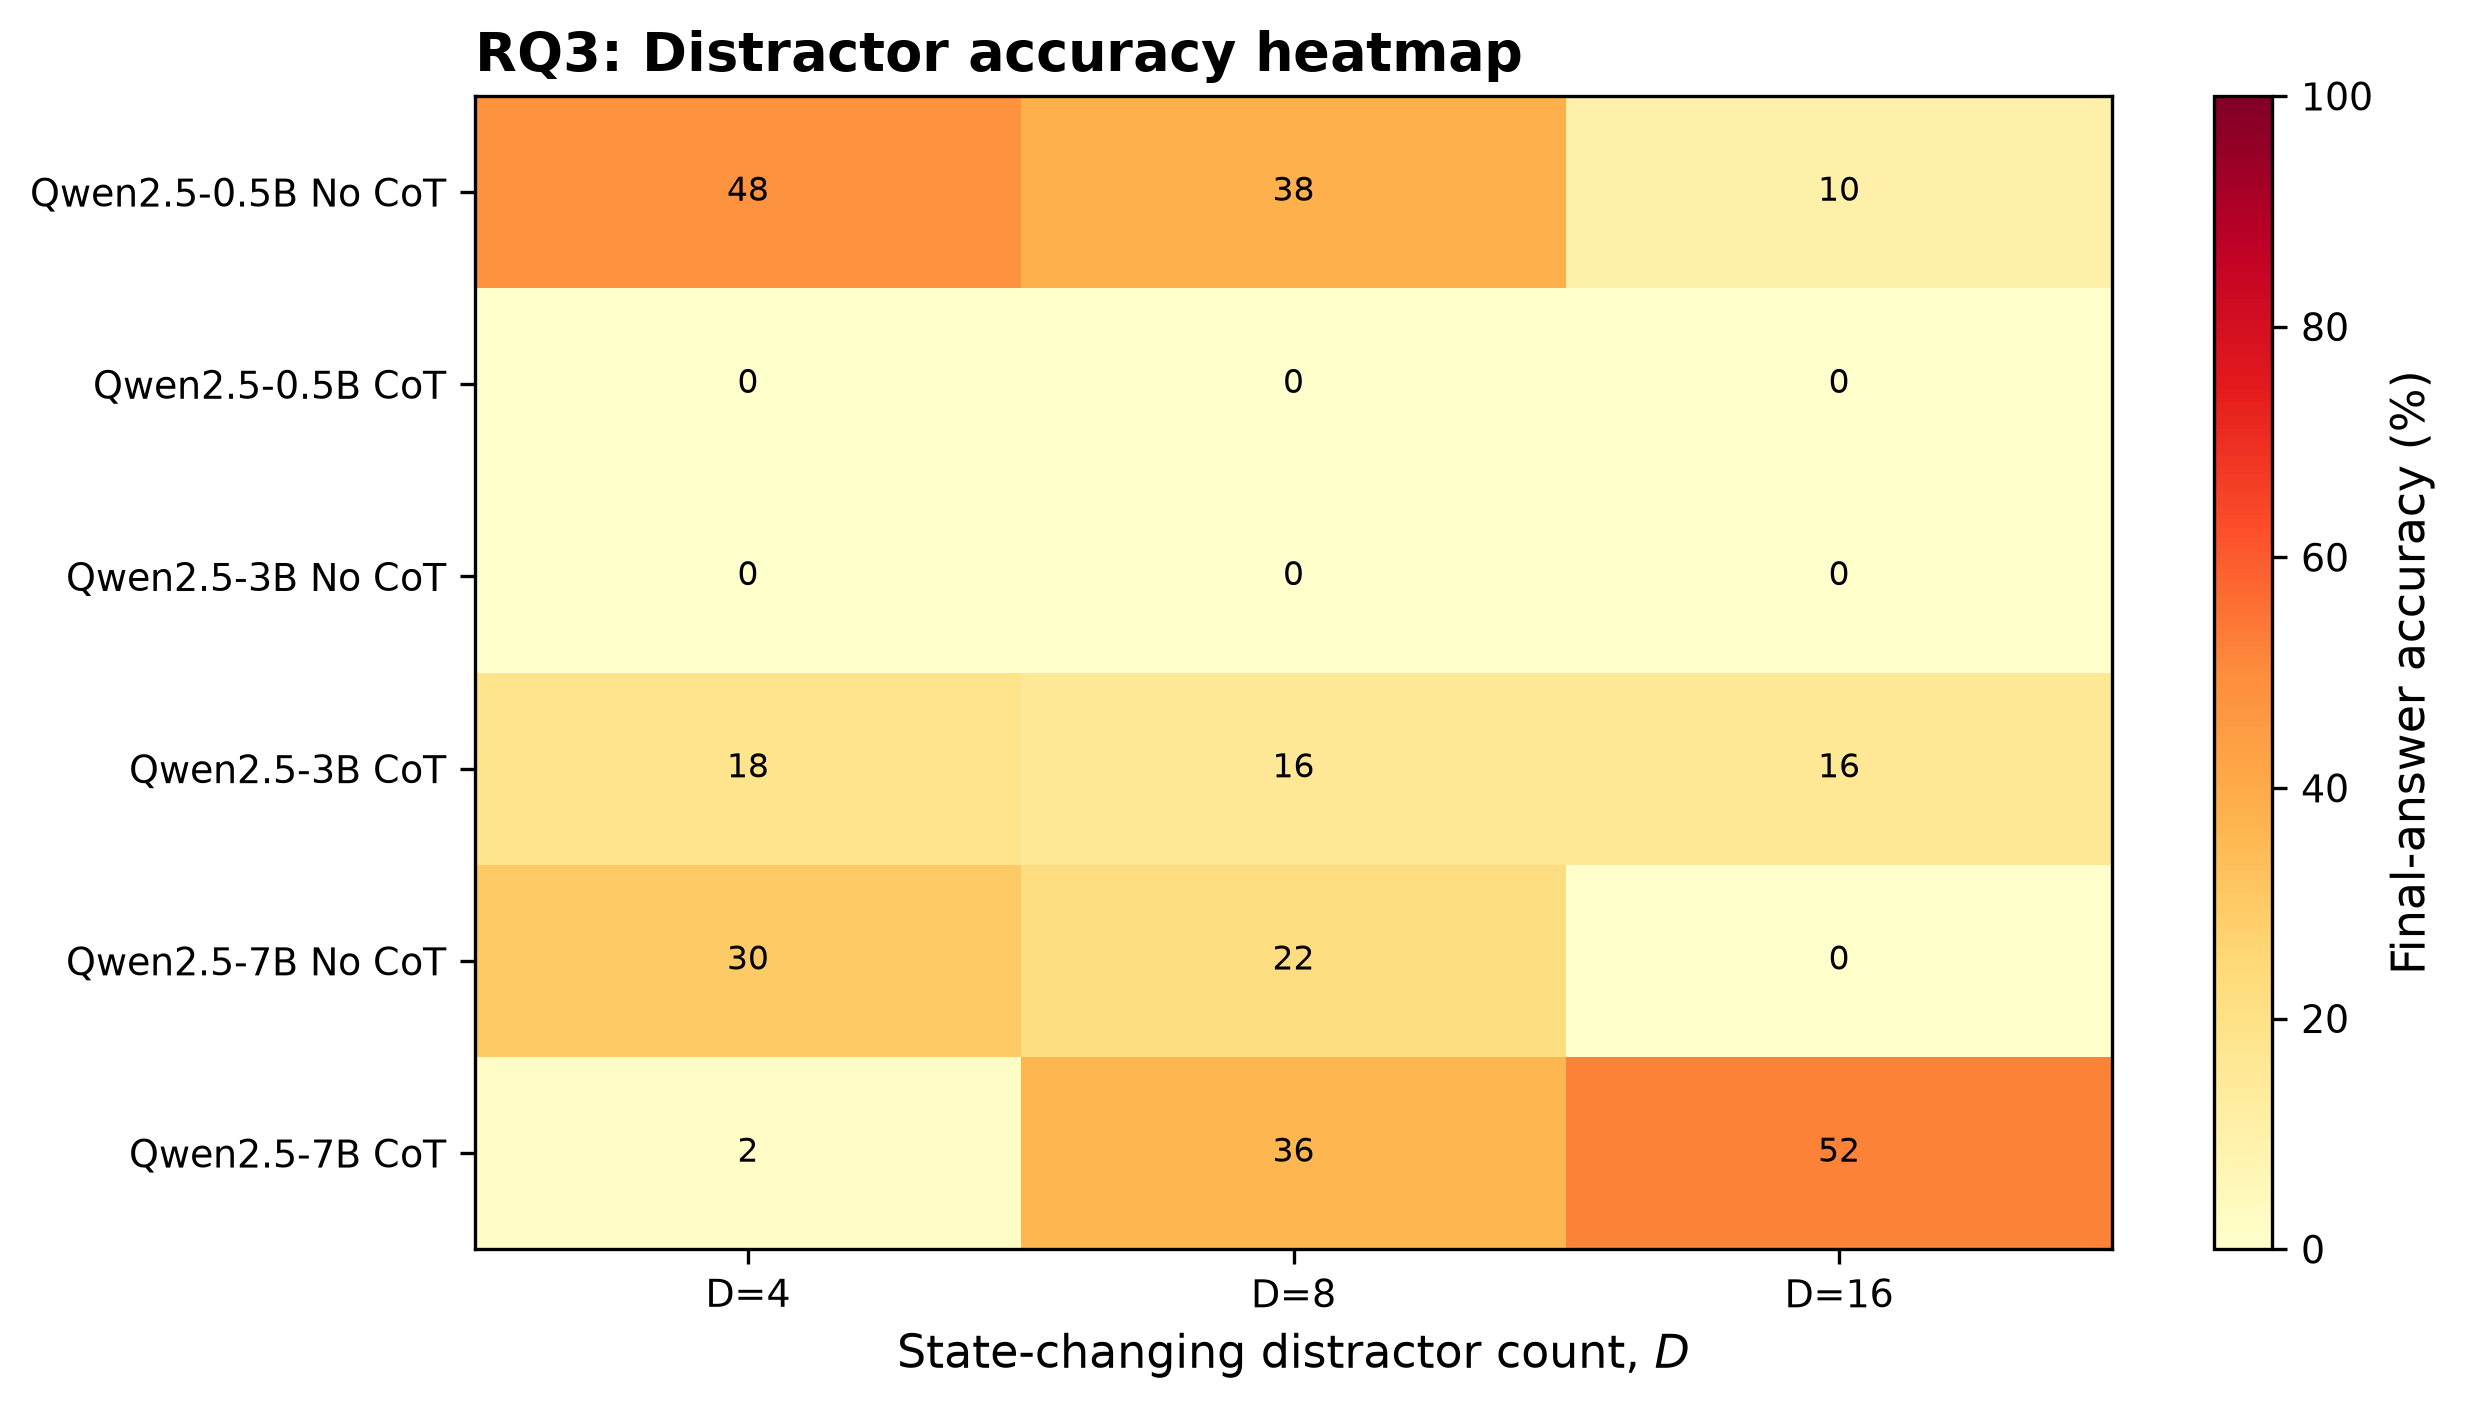
\includegraphics[width=\textwidth]{fig04_rq3_distractor_heatmap.png}
\caption{RQ3 final-answer accuracy across state-changing distractor counts and model-prompting configurations.}
\label{fig:rq3-distractor-heatmap}
\end{figure}

The distractor sweep demonstrates that the benchmark is sensitive to irrelevant state updates, but the
pattern is model- and prompting-dependent rather than uniformly monotonic. The 0.5B model without CoT
falls to 29\% at $D=4$ and 10\% at $D=16$, while the 3B configurations remain broadly low across all
three distractor conditions. The 0.5B CoT variant fails completely on the distractor sweep, and the 7B CoT
variant improves from 7\% at $D=4$ to 52\% at $D=16$. These findings provide evidence of sensitivity to
state-changing interference, but they do not support a uniform degradation pattern across models.

\section{RQ4 Results: Entity Load}
The dedicated entity-load sweep was generated as part of the benchmark, but the repository's available
model-output artifacts do not yet include the corresponding evaluated RQ4 summaries. This condition
therefore remains an active part of the evaluation plan rather than a completed empirical finding.

\section{RQ5 Results: Structural Operation Pilot}
The structural-operation pilot contains 250 instances: 50 instances in each of the five operation
families. These records are included in the 1,150-instance benchmark evaluated by all six
model-prompting configurations; they are not an additional 500-instance dataset. The \texttt{split\_chain}
records realize $T_{\mathrm{actual}}=7$ and $D_{\mathrm{actual}}=1$, while the available records for the other four
families realize $T_{\mathrm{actual}}=8$. The resulting family-level final-answer accuracies are:

\begin{table}[H]
\centering
\begin{tabularx}{\textwidth}{Xccccc}
\toprule
\textbf{Model / Prompting} & \textbf{Split} & \textbf{Merge} & \textbf{Swap} & \textbf{Undo} & \textbf{Undo--Redo} \\
\midrule
Qwen2.5-0.5B, No CoT & 12.0\% & 68.0\% & 56.0\% & 60.0\% & 68.0\% \\
Qwen2.5-0.5B, CoT & 0.0\% & 0.0\% & 0.0\% & 0.0\% & 0.0\% \\
Qwen2.5-3B, No CoT & 8.0\% & 18.0\% & 20.0\% & 58.0\% & 80.0\% \\
Qwen2.5-3B, CoT & 66.0\% & 92.0\% & 18.0\% & 92.0\% & 64.0\% \\
Qwen2.5-7B, No CoT & 0.0\% & 0.0\% & 8.0\% & 0.0\% & 0.0\% \\
Qwen2.5-7B, CoT & 8.0\% & 6.0\% & 6.0\% & 2.0\% & 4.0\% \\
\bottomrule
\end{tabularx}
\caption{Final-answer accuracy for the five structural-operation families in RQ5. Each cell is based on 50 instances.}
\label{tab:rq5-results}
\end{table}

The results show operation-specific variation rather than a uniform structural-operation difficulty.
Qwen2.5-3B with CoT performs strongly on merge and undo, but much less strongly on swap. The same
model without CoT performs best on undo-redo, while the 0.5B CoT and 7B configurations remain weak
across nearly all families. Because the split family has a different realized target depth, these
family comparisons should be interpreted descriptively rather than as perfectly matched causal contrasts.

\begin{figure}[H]
\centering
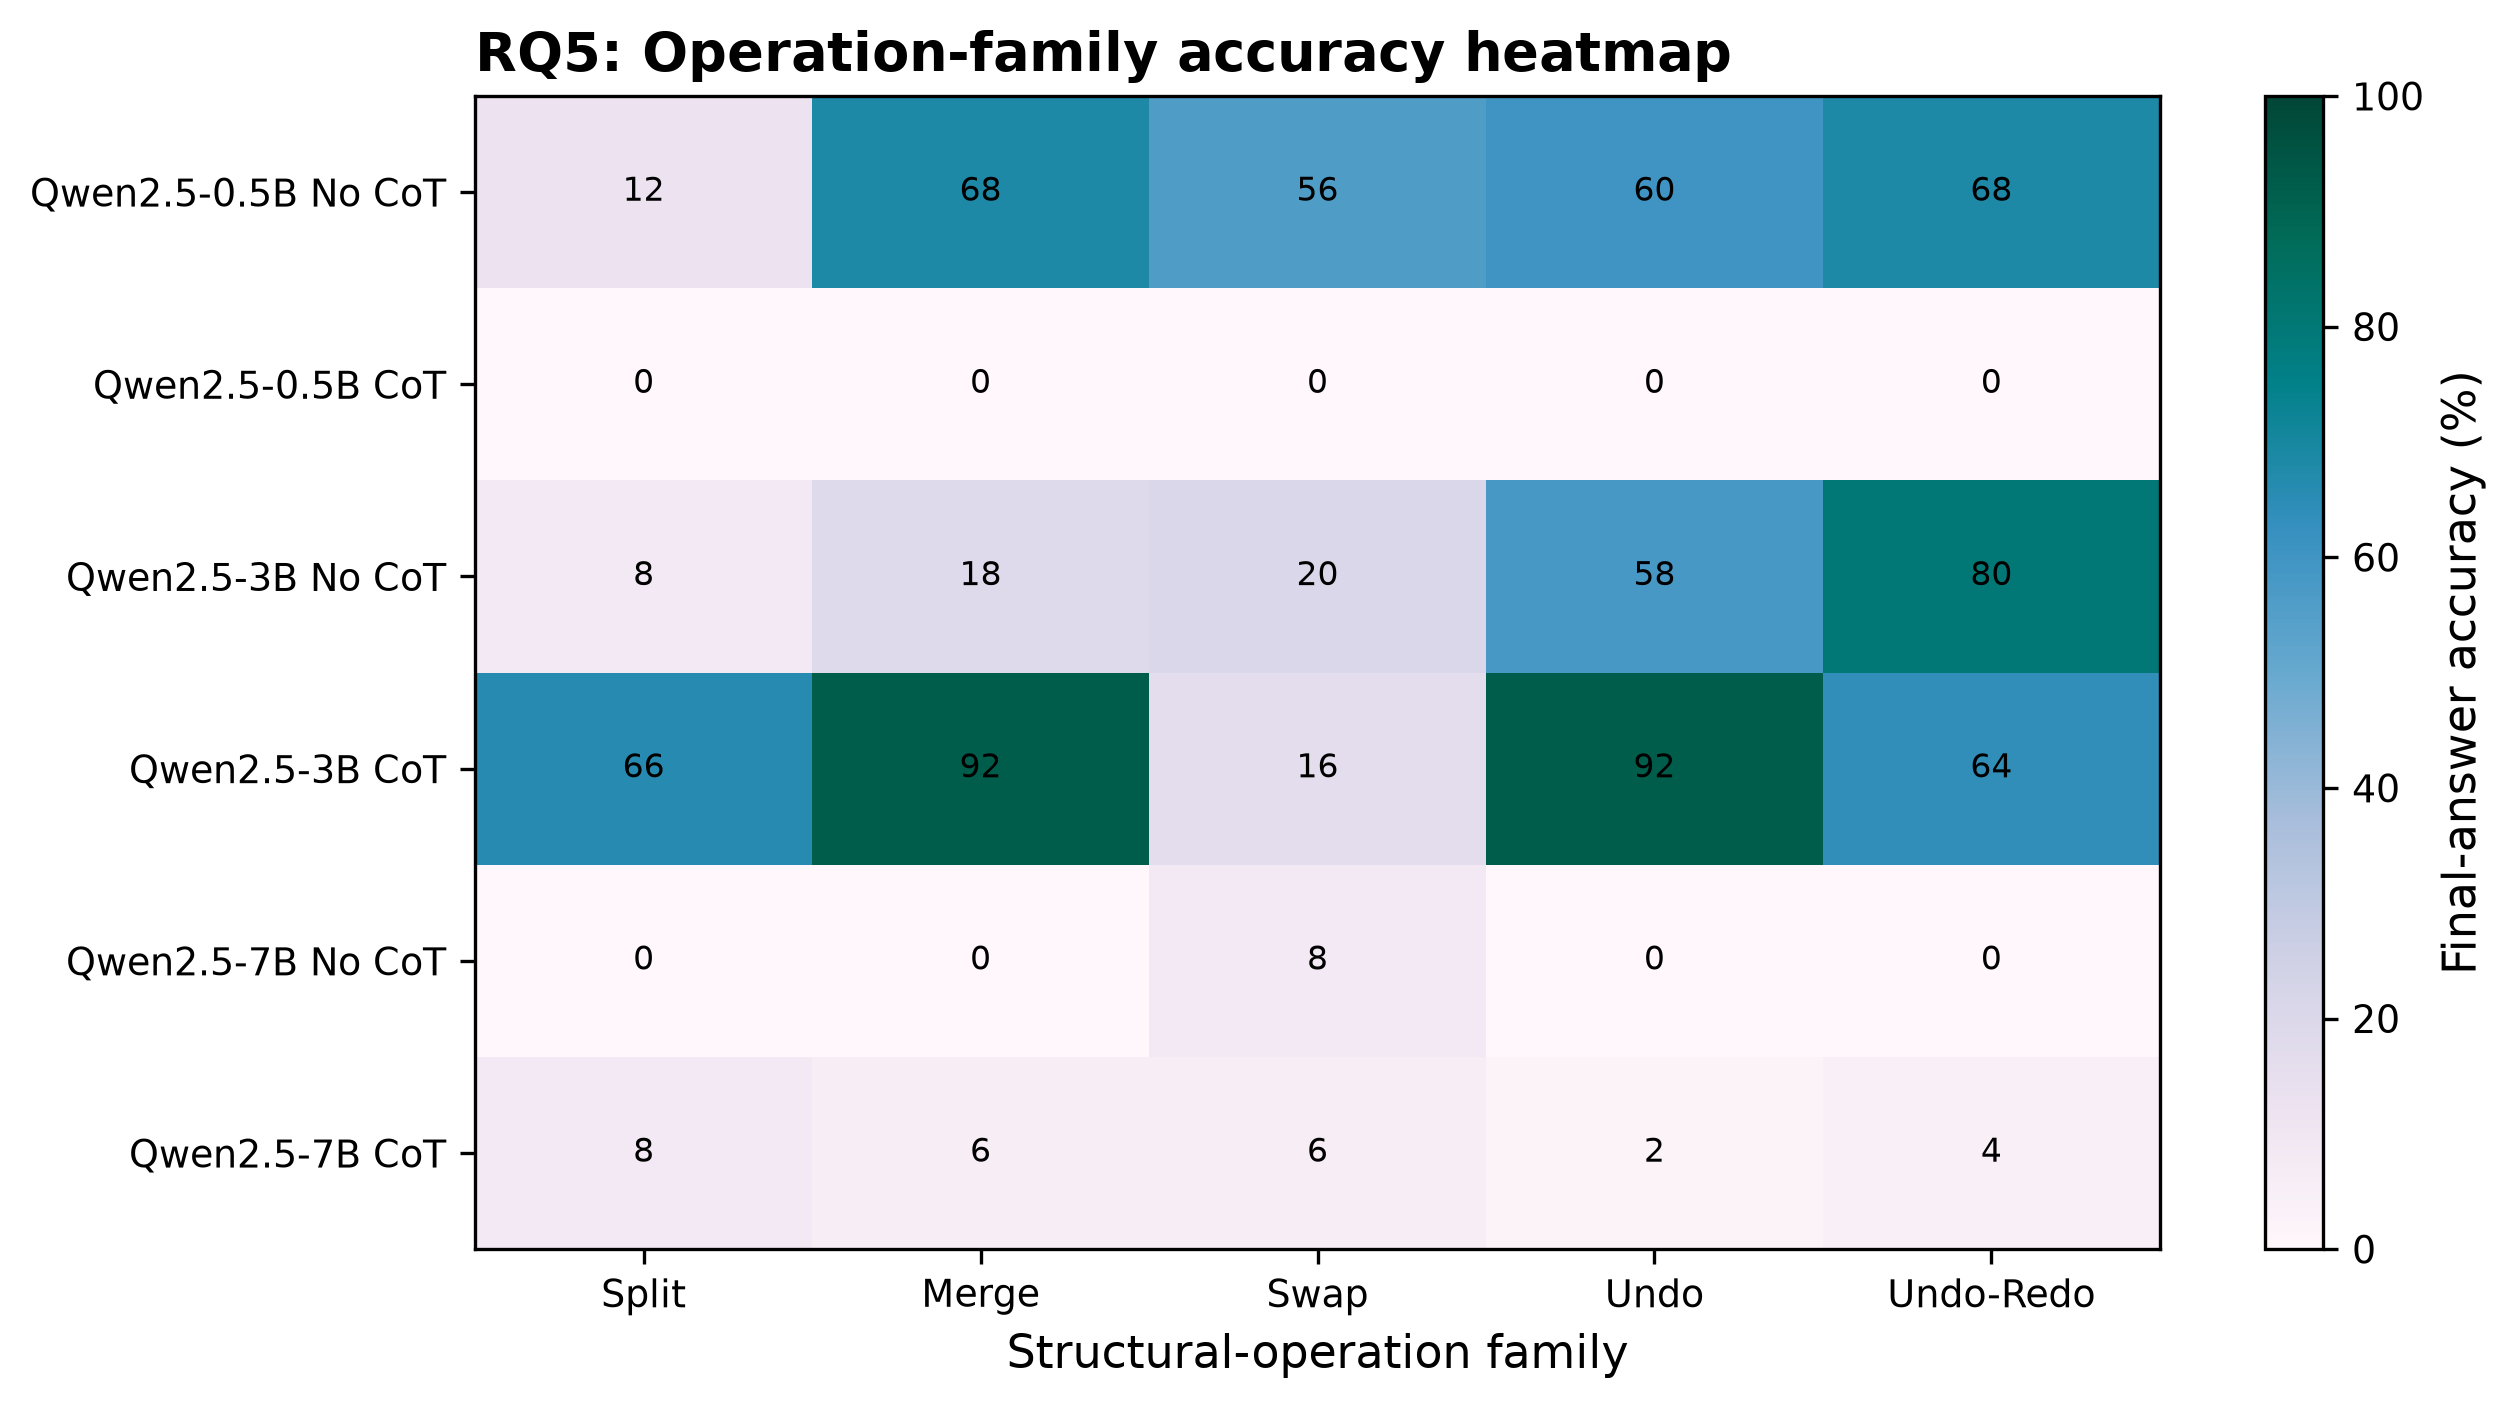
\includegraphics[width=\textwidth]{fig06_rq5_operation_heatmap.png}
\caption{RQ5 final-answer accuracy across structural-operation families and model-prompting configurations.}
\label{fig:rq5-operation-heatmap}
\end{figure}

\section{Performance-Degradation and Error-Dynamics Analysis}
The observed degradation curves are consistent with a vulnerability in maintaining relevant state
information as the number of updates increases and as competing transitions are introduced. For the 0.5B
model, early degradation appears between $T=2$ and $T=6$, while the revision and distractor sweeps show a
sharp decline in several configurations. The 3B model is more robust on clean depth tracking but still
fails sharply on revision and distractor conditions. These patterns are consistent with state-maintenance
difficulty under interference and revision, although the behavioral evidence alone does not establish the
underlying internal mechanism.

The evaluation reports further distinguish between final-answer errors and step-wise state errors. In the
repository outputs, step-wise accuracies remain notably lower than final-answer accuracy in several cases,
which indicates that many model responses do not preserve intermediate state consistency even when they
produce a plausible final answer. This pattern is consistent with the benchmark's emphasis on canonical
state tracking across the whole trajectory rather than isolated final-query retrieval.

\begin{figure}[H]
\centering
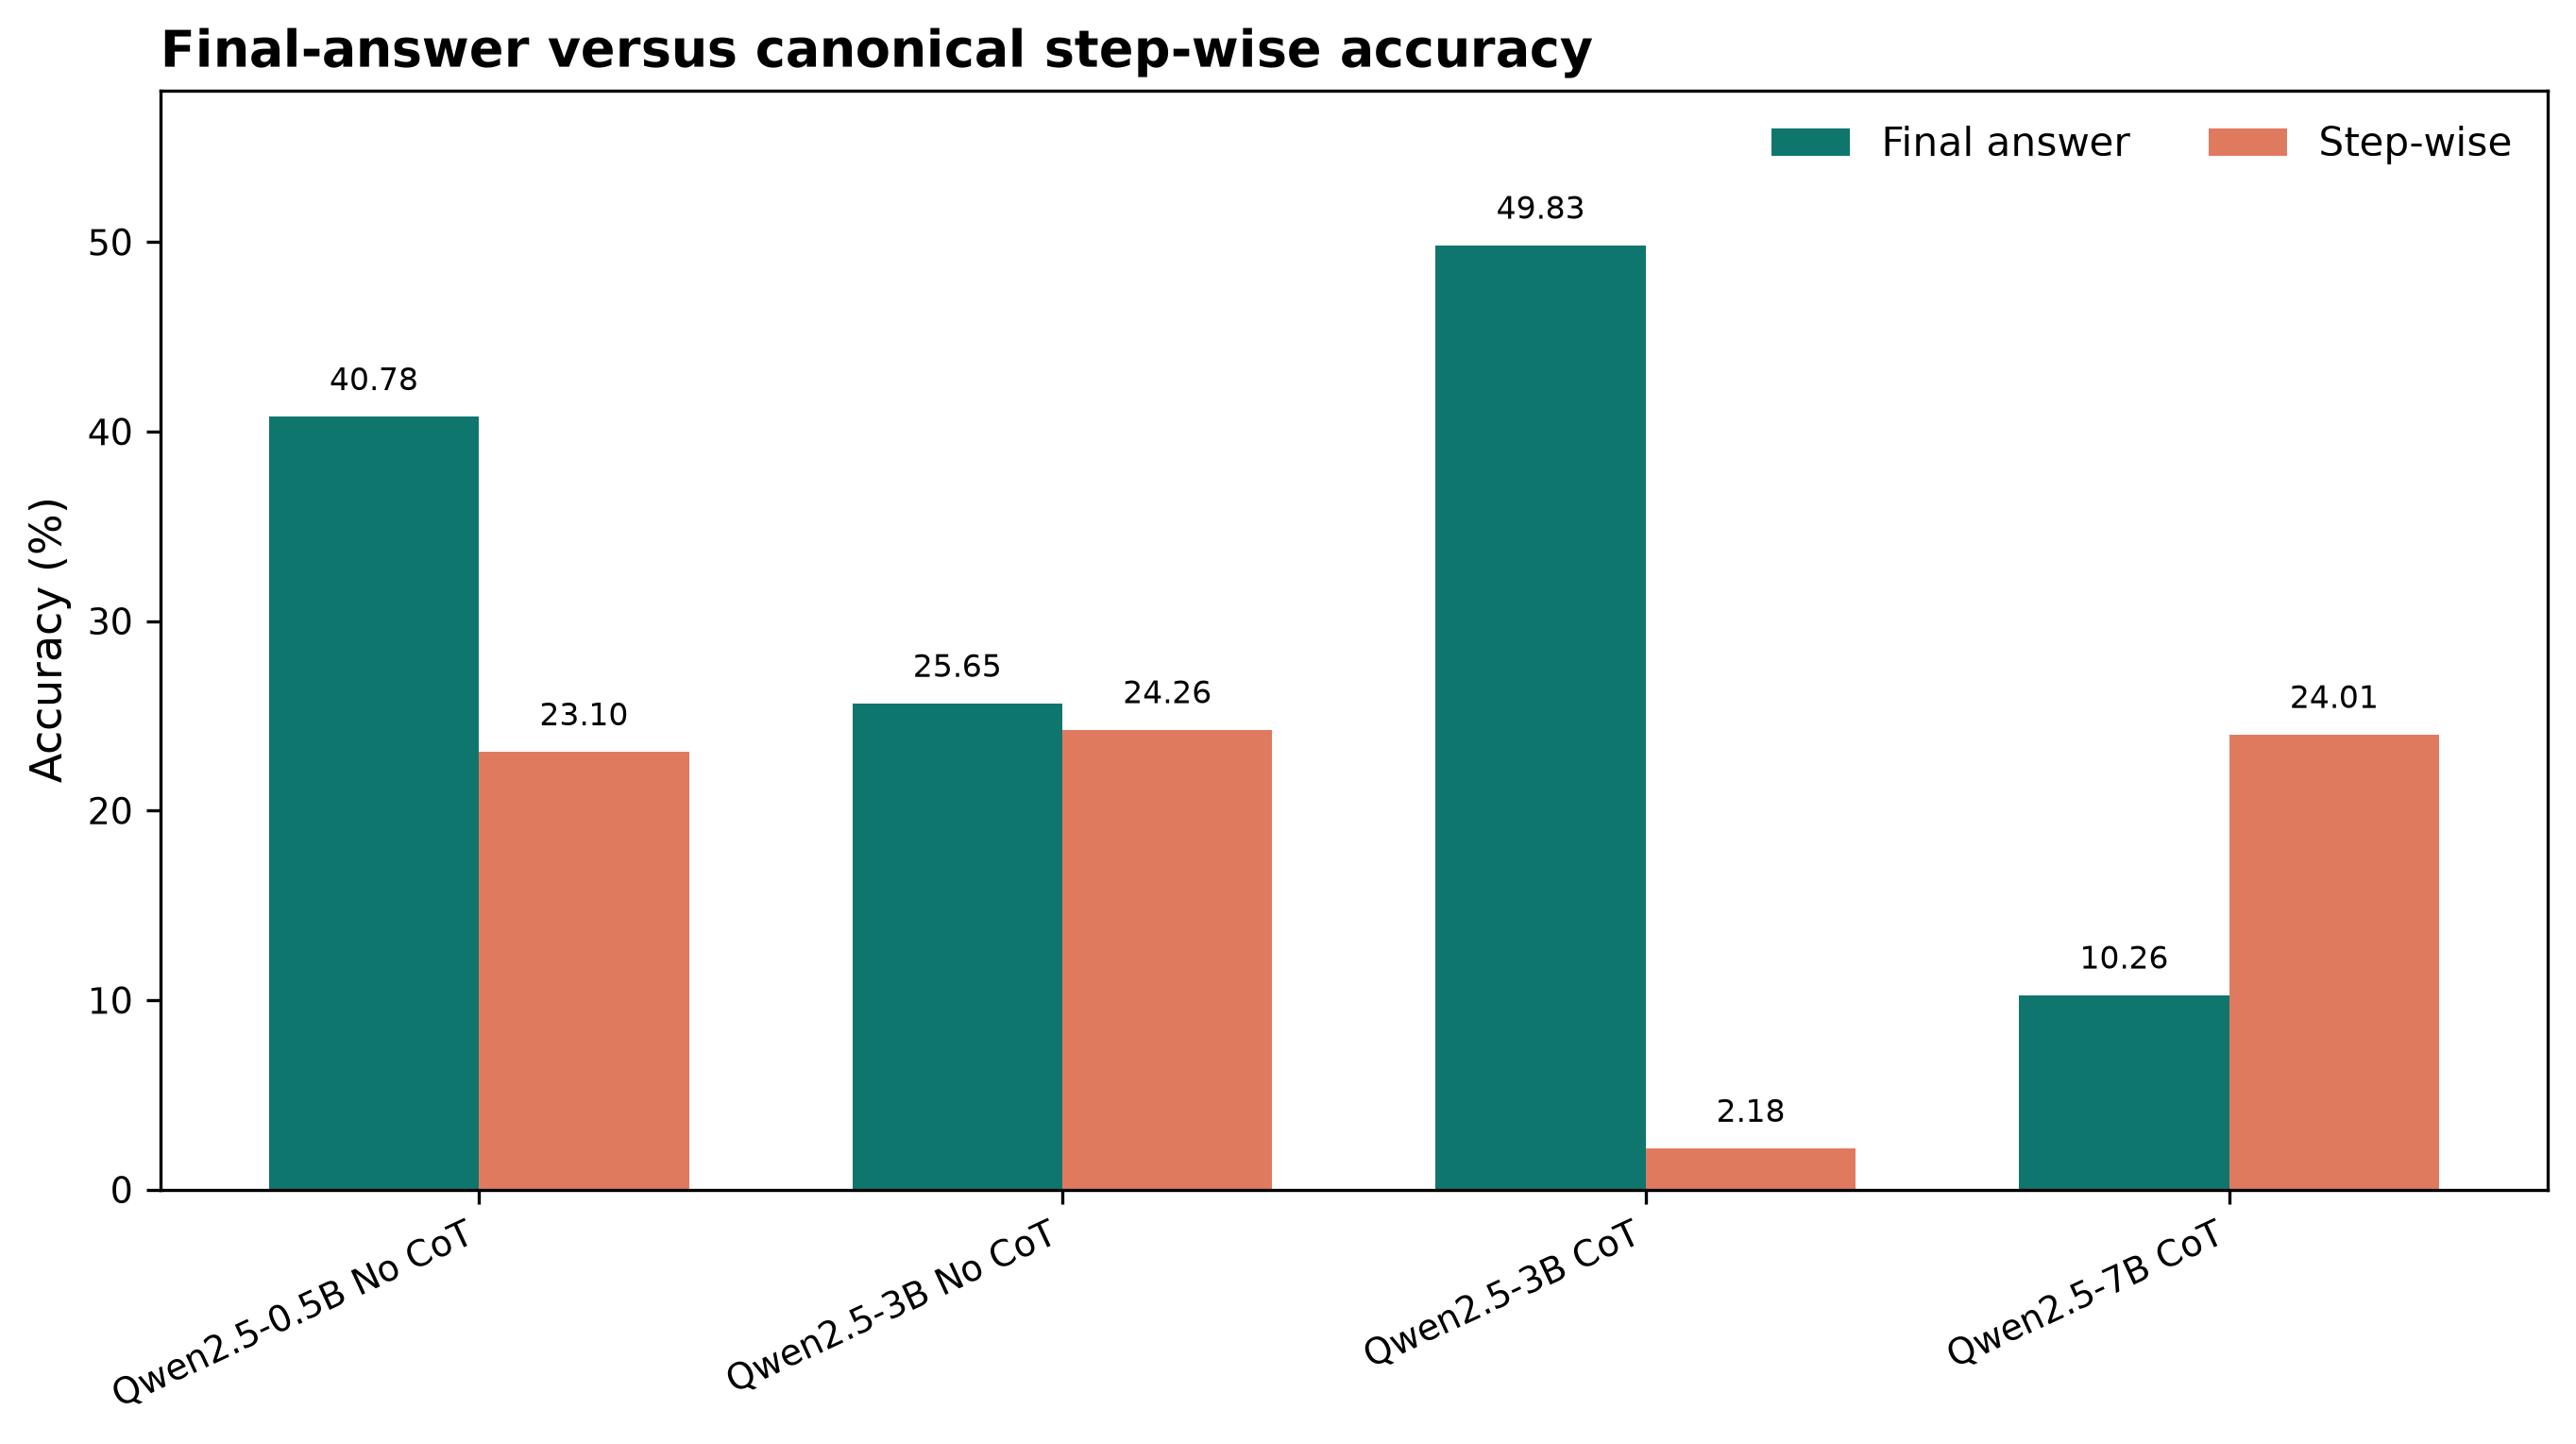
\includegraphics[width=\textwidth]{fig05_final_vs_stepwise.png}
\caption{Comparison of final-answer and step-wise accuracy across the evaluated model-prompting configurations.}
\label{fig:final-vs-stepwise}
\end{figure}

\section{Phase 3: Naturalistic Reference Audit Status}
The naturalistic reference set is reported separately from the controlled benchmark. No model-level
results are included in the current evaluation artifacts, so this phase remains exploratory and does not
contribute an empirical claim to the main conclusions. Because a naturalistic corpus would not maintain
the same explicit experimental isolation as DWS-Bench, any future observations would be descriptive rather
than causal.

\section{Research Question Summary}
The empirical findings across the available model reports can be summarized as follows.

\begin{table}[H]
\centering
\begin{tabular}{p{0.16\textwidth}p{0.68\textwidth}}
\toprule
\textbf{RQ} & \textbf{Empirical Finding} \\
\midrule
RQ1 & Temporal depth substantially affects performance in some configurations, but the observed relationship is non-monotonic. The 0.5B model without CoT falls from 100\% at $T=2$ to 24\% at $T=6$, while the 3B model with CoT remains highly accurate through $T=12$ before declining at $T=16$. \\
RQ2 & Revision complexity creates a substantial but highly configuration-dependent failure mode. The 0.5B No-CoT configuration declines from 48\% at $T=4$ to 30\% at $T=16$, while the 3B CoT configuration is highly unstable, reaching 76\% at $T=8$ but only 2--6\% at the other tested depths. \\
RQ3 & State-changing distractor effects are strongly model- and prompting-dependent. The 0.5B No-CoT configuration falls to 10\% at $D=16$, whereas the 7B CoT configuration increases from 7\% to 52\%. The results establish sensitivity to distractor structure but not a uniform monotonic degradation pattern. \\
RQ4 & Entity-load analysis is generated but not yet present in the repository's model-output artifacts. \\
RQ5 & The five structural-operation families are represented by 250 evaluated records within the 1,150-instance benchmark. Results vary substantially by operation, model, and prompting condition. \\
\bottomrule
\end{tabular}
\caption{Summary of the empirical findings tied to the research questions.}
\label{tab:rq-summary}
\end{table}

\chapter{Ethical, Social, and Environmental Considerations}
\section{Data Integrity}
DWS-Bench uses synthetic benchmark data. No personal or sensitive data are required for the core
benchmark.

The primary integrity mechanism is the strict separation between symbolic ground truth and natural-language rendering.

The generation process is:
\[
\text{Symbolic State}
\rightarrow
\text{Validation}
\rightarrow
\text{Natural Language}.
\]
The reverse process is never used to determine the ground-truth answer.

Consequently, a natural-language generation error does not alter the authoritative answer stored by the
benchmark.

\section{Reproducibility and Research Ethics}
The benchmark conditions, random seeds where applicable, validation results, and model configurations
are recorded in the associated experiment artifacts.

Results should be reported for all predefined conditions, including conditions in which model
performance is poor.

No experimental condition should be removed solely because it produces an unfavorable result.

\section{Social Accessibility}
Small Language Models can reduce the computational requirements associated with AI deployment.
This can be particularly relevant for resource-constrained environments, edge devices, educational
infrastructure, and offline systems.

However, smaller models may also exhibit greater limitations in complex reasoning tasks. DWS-Bench
therefore provides a mechanism for identifying such limitations rather than assuming that lower
computational cost implies equivalent reasoning capability.

\section{Environmental Sustainability}
The benchmark uses synthetic data generation and deterministic symbolic simulation, which require
substantially fewer resources than manually annotating large datasets.

The evaluation of smaller models may also reduce inference requirements compared with evaluating
very large models.

However, the environmental impact of the benchmark is not assumed to be zero. Model inference
consumes computational resources. The current evaluation records the model configurations and
benchmark size; exact energy consumption was not measured, so no direct carbon estimate is claimed.

% =================================================================
% CHAPTER 9 -- CHALLENGES AND LIMITATIONS
% =================================================================
\chapter{Challenges and Limitations}
\section{Factor Confounding}
The benchmark explicitly measures multiple complexity factors, but measurement does not guarantee
perfect independence. In particular, deeper trajectories and larger numbers of updates can produce
longer rendered narratives. The benchmark reduces this coupling through matched rendered lengths and
length-only controls, as described in the experimental-contract chapter. The current analysis does not
provide a complete multivariate adjustment for every factor simultaneously.

These mechanisms reduce, but do not eliminate, residual confounding. Length-matching trades one
coupling for another, and the length-only control measures the remaining length effect directly.
Causal interpretation of any single factor therefore remains subject to the residual associations
that the realized factor measurements expose.


\section{Synthetic Benchmark Assumptions}
DWS-Bench provides strong control over symbolic state and experimental factors, but synthetic worlds
cannot reproduce all properties of real-world reasoning. Naturalistic tasks may contain ambiguity,
incomplete observations, implicit relations, commonsense requirements, and linguistic variation that
are absent from the controlled benchmark.

\section{Operation-Semantics Coverage}
The current implementation includes eight operation types, but the vocabulary still represents only a
subset of dynamic reasoning patterns. Additional relations, nested structures, and more complex
multi-entity transformations may introduce failure modes not captured by the present benchmark.

\section{Model Coverage}
The evaluation covers three instruction-tuned Qwen2.5 parameter-scale variants and several parameter
scales. This provides a useful comparative sample but does not establish generalization to all SLM
architectures, training corpora, quantization schemes, or inference configurations.

\section{Prompt and Inference Effects}
Model behavior can depend on prompt wording, demonstrations, decoding settings, and reasoning
instructions. The controlled evaluation fixes these choices within the study, but the results should
not be interpreted as invariant to all possible prompting or inference configurations.

\section{Naturalistic Transfer}
The naturalistic reference set is intentionally secondary and has no model-level results in the current
artifacts. It therefore contributes no empirical transfer claim and cannot support the same causal
conclusions as the controlled experiments.

\section{Benchmark Selection Effects}
QuerySpec-based generation improves structural control but also imposes a selection criterion on the
space of possible trajectories. Consequently, the benchmark characterizes the behavior of models on
the selected controlled families rather than on every possible dynamic world-state narrative.

\chapter{Conclusion and Future Work}
\section{Conclusion}
This thesis presents DWS-Bench, a controlled benchmark for evaluating dynamic world-state reasoning in
Small Language Models. The benchmark is designed around a central methodological principle: the
underlying state trajectory must be specified and validated independently of its natural-language
realization.

The system constructs symbolic trajectories, applies deterministic state transitions, and uses a
QuerySpec-based structural analysis layer to select instances satisfying explicit experimental
requirements. A separate renderer converts validated trajectories into natural-language narratives,
while the evaluator compares model predictions against canonical symbolic states.

The benchmark measures target-relevant temporal depth, state revision, distractor interference,
narrative distractors, entity load, and other realized properties of the generated instances. Rather
than assuming that these factors are perfectly independent, the benchmark records their actual values
and inspects residual associations before the model-evaluation phase.

The evaluation is organized into five research questions. RQ1 investigates temporal depth and
substantial degradation; RQ2 investigates state revision; RQ3 investigates distractor interference;
RQ4 investigates entity load; and RQ5 investigates structural-operation families. Three instruction-
tuned Small Language Models are evaluated using final-answer accuracy and, for configurations with
available canonical intermediate-state outputs, step-wise accuracy. The naturalistic reference set is
treated as exploratory because no model-level audit results are stored.

The empirical results show that the benchmark is sensitive to temporal depth, revision, and distractor
interference, but the effect is highly model- and prompting-dependent. Across the three evaluated models,
Qwen2.5-3B with CoT performs best overall, while the 0.5B CoT configuration fails almost completely on the
benchmark. Among the configurations for which both metrics are available, the strongest observed discrepancy
occurs for the 3B CoT model, where final accuracy reaches 49.91\% but step-wise accuracy remains only 2.82\%.
This pattern shows that final-answer correctness can coexist with poor agreement with the canonical
intermediate states. It suggests that final-answer accuracy alone may not adequately characterize
trajectory-level state tracking, although the behavioral results do not establish the model's internal
mechanism. RQ4 remains unevaluated at the model-output level, while RQ5 has completed family-level
model evaluation within the 1,150-instance benchmark.

\section{Future Work}
Future extensions include:
\begin{enumerate}
\item broader query types and multi-object questions;
\item containment, ownership, and additional relational state representations;
\item richer multi-hop and multi-entity reasoning;
\item longer and more varied dependency structures;
\item broader model and parameter-scale coverage;
\item representation-level and mechanistic analysis of state tracking;
\item additional naturalistic datasets and transfer settings;
\item improved statistical controls for residual context-length confounding;
\item expanded trajectory families and operation semantics.
\end{enumerate}

\begin{appendices}
\chapter{Weekly Meeting Summaries}
The following table records weekly progress, decisions, and planned work, reconstructed from the
team's WhatsApp group log (``Batch 22 -- Thesis group'').

\begingroup
\small
\begin{longtable}{@{}p{0.04\textwidth}p{0.10\textwidth}p{0.22\textwidth}p{0.22\textwidth}p{0.22\textwidth}@{}}
\caption{Weekly meeting summaries and project progress.}
\label{tab:weekly-summary}\\
\hline
\textbf{No.} & \textbf{Date} & \textbf{Progress / Contribution} & \textbf{Decision / Discussion} &
\textbf{Next Plan} \\
\hline
\endfirsthead

\multicolumn{5}{l}{\small\textit{(continued from previous page)}} \\
\hline
\textbf{No.} & \textbf{Date} & \textbf{Progress / Contribution} & \textbf{Decision / Discussion} &
\textbf{Next Plan} \\
\hline
\endhead

\hline
\multicolumn{5}{r}{\small\textit{(continued on next page)}} \\
\endfoot

\hline
\endlastfoot

1 & 14--18 May 2026 &
Started literature review on LLM interpretability and concept representations. Set up the thesis GitHub
repository. &
Discussed LRH, CRH, steering vectors, and their limitations. &
Read background papers and prepare for supervisor discussion. \\
\hline
2 & 20--22 May 2026 &
Reviewed additional papers shared by the supervisor. &
Discussed the need to understand the papers before selecting a research direction. &
Review the remaining papers and identify possible research gaps. \\
\hline
3 & 28 May--02 June 2026 &
Continued literature review; supervisor shared work on LLM working memory. &
Working memory and reasoning became potential areas of interest. &
Continue literature review and arrange the next meeting. \\
\hline
4 & 03--05 June 2026 &
Coordinated and attended a supervisor meeting. &
Discussed the team's progress and ongoing literature exploration. &
Continue narrowing down the research direction. \\
\hline
5 & 10--12 June 2026 &
Progress was temporarily limited due to ML coursework and quizzes. &
Meeting was postponed with supervisor approval. &
Resume thesis work after academic deadlines. \\
\hline
6 & 14--17 June 2026 &
Prepared to discuss accumulated literature findings with the supervisor. &
Meeting was arranged to review progress and possible research directions. &
Present findings and identify a feasible research problem. \\
\hline
7 & 14--15 July 2026 &
Converged toward SLM reasoning and state-tracking evaluation. Draft proposal was shared. &
Identified a possible gap in multi-parameter evaluation of SLM state tracking. Proposed adapting Kim
\& Schuster's (ACL 2023) entity-tracking generator. &
Refine the research gap and benchmark design. \\
\hline
8 & 17--23 July 2026 &
Continued refining the SLM state-tracking proposal after a postponed meeting. &
Supervisor meeting was rescheduled. &
Discuss the benchmark and research gap in detail. \\
\hline
9 & 23--31 July 2026 &
Refined the project toward a controlled dynamic world-state benchmark. &
Discussed using a deterministic simulator and controllable task parameters. &
Formalize the variables and begin implementation. \\
\hline
10 & 03 August 2026 &
Continued literature review and benchmark methodology development. &
Focused on isolating different sources of difficulty in SLM state tracking. &
Implement the deterministic state-generation and validation pipeline. \\
\hline
11 & 09--14 August 2026 &
Formalized the symbolic-simulator-first approach and experimental variables. &
Ground truth should be generated independently from natural-language rendering. &
Test alternative rendering approaches on a small pilot set. \\
\hline
12 & 15 August 2026 &
Discussed deterministic question generation versus LLM-based paraphrasing. Reviewed related task
formulations such as LinearWorld, HandSwap, and Lights. &
Supervisor recommended testing both approaches at small scale. Team considered deterministic
variation preferable due to lower risk of ground-truth drift. &
Run a small comparison and finalize the rendering strategy. \\
\hline
\end{longtable}
\endgroup

% -----------------------------------------------------------------
% APPENDIX B -- IMPLEMENTATION AND GITHUB ARTIFACTS
% -----------------------------------------------------------------
\chapter{Implementation and GitHub Artifacts}
\section{Repository Structure}
The final repository should contain the following logical components:
\begin{table}[H]
\centering
\begin{tabular}{ll}
\toprule
\textbf{Component} & \textbf{Responsibility} \\
\midrule
Contract & Experimental condition specification \\
Generator & Symbolic trajectory construction \\
Validator & Constraint and state validation \\
Sampler & Controlled instance generation \\
Renderer & Natural-language rendering \\
Evaluator & SLM inference and metric computation \\
Tests & Unit, smoke, and robustness tests \\
\bottomrule
\end{tabular}
\caption{Required repository components.}
\label{tab:repository-components}
\end{table}

\section{Technical Contribution Matrix}
Each member must provide two distinct Pull Request identifiers and a specific technical contribution.
\begin{table}[H]
\centering
\small
\renewcommand{\arraystretch}{1.4}
\begin{tabular}{|p{0.22\textwidth}|p{0.12\textwidth}|p{0.5\textwidth}|}
\hline
\textbf{Member} & \textbf{PR ID} & \textbf{Technical Contribution} \\
\hline
MD.Mahiul Kabir & -- & Symbolic World Simulator and Experimental Contract implementation. \\
\hline
MD.Mahiul Kabir & -- & Repository artifact documentation and implementation validation. \\
\hline
Rahatut Tahrim Mounota & -- & Trajectory Generator and Validation Logic implementation. \\
\hline
Rahatut Tahrim Mounota & -- & Benchmark validation and result-aggregation support. \\
\hline
Nayeemul Hasan Prince & -- & Natural-Language Renderer and Prompt Generation. \\
\hline
Nayeemul Hasan Prince & -- & Report synthesis and evidence-alignment review. \\
\hline
\end{tabular}
\caption{Technical contribution matrix.}
\label{tab:technical-contributions}
\end{table}
\normalsize

\section{GitHub Contribution Metrics}
The final report must contain actual repository statistics.
\begin{table}[H]
\centering
\begin{tabular}{p{0.28\textwidth}p{0.17\textwidth}p{0.17\textwidth}p{0.17\textwidth}}
\toprule
\textbf{Member} & \textbf{Commits} & \textbf{Additions} & \textbf{Deletions} \\
\midrule
MD.Mahiul Kabir & -- & -- & -- \\
Rahatut Tahrim Mounota & -- & -- & -- \\
Nayeemul Hasan Prince & -- & -- & -- \\
\midrule
\textbf{Total} & -- & -- & -- \\
\bottomrule
\end{tabular}
\caption{GitHub contribution statistics.}
\label{tab:github-metrics}
\end{table}

\section{Pull Request Verification}
The final version must verify two distinct PRs for every team member.
\begin{table}[H]
\centering
\begin{tabular}{p{0.28\textwidth}p{0.27\textwidth}p{0.27\textwidth}}
\toprule
\textbf{Member} & \textbf{PR 1} & \textbf{PR 2} \\
\midrule
MD.Mahiul Kabir & -- & -- \\
Rahatut Tahrim Mounota & -- & -- \\
Nayeemul Hasan Prince & -- & -- \\
\bottomrule
\end{tabular}
\caption{Pull Request verification matrix.}
\label{tab:pr-verification}
\end{table}

% -----------------------------------------------------------------
% APPENDIX C -- FINAL COMPLIANCE AUDIT
% -----------------------------------------------------------------
\chapter{Final Compliance Audit}
The following checklist should be completed before final submission.
\begin{table}[H]
\centering
\small
\renewcommand{\arraystretch}{1.4}
\begin{tabular}{|p{0.12\textwidth}|p{0.62\textwidth}|p{0.12\textwidth}|}
\hline
\textbf{State} & \textbf{Requirement} & \textbf{Status} \\
\hline
\textbf{Done} & Chapters 1--10 contain complete methodological and empirical content. & Completed \\
\hline
\textbf{Done} & Phase 1 generator validation and factor-distribution analysis completed. & Completed \\
\hline
\textbf{Done} & Realized factor associations have been inspected before benchmark freezing. & Completed \\
\hline
\textbf{Done} & Frozen benchmark datasets are used for Phase 2 evaluation. & Completed \\
\hline
\textbf{Done} & Three target SLMs have been evaluated under the fixed protocol. & Completed \\
\hline
\textbf{Done} & Final-answer and step-wise accuracy are reported. & Completed \\
\hline
\textbf{Done} & RQ1--RQ3 results and interpretations are reported. & Completed \\
\hline
\textbf{Open} & RQ4 evaluation remains pending. & Pending \\
\hline
\textbf{Done} & RQ5 structural-operation families are generated, validated, and evaluated within the core benchmark. & Completed \\
\hline
\textbf{Done} & Performance-degradation and error-dynamics analyses are reported. & Completed \\
\hline
\textbf{Open} & Naturalistic reference audit is documented as a secondary analysis. & Pilot / Descriptive \\
\hline
\textbf{Done} & Symbolic ground truth is independent of the natural-language renderer. & Completed \\
\hline
\textbf{Done} & Validator performs the mandatory structural and state-consistency checks. & Completed \\
\hline
\textbf{Done} & Appendix A contains weekly meeting summaries. & Completed \\
\hline
\textbf{Open} & Appendix B contains project and GitHub artifacts. & Pending final artifact verification \\
\hline
\textbf{Open} & GitHub contribution evidence is included where required. & Pending final artifact verification \\
\hline
\textbf{Done} & Chapter~\ref{chap:results} contains findings linked explicitly to each research question. & Completed \\
\hline
\end{tabular}
\caption{Final DWS-Bench compliance audit checklist.}
\label{tab:final-audit}
\end{table}
\normalsize

\section{Final Presentation Requirements}
The final presentation should explicitly communicate:
\begin{enumerate}
\item the DWS-Bench architecture;
\item the QuerySpec and experimental contract;
\item the eight-operation capability taxonomy;
\item Phase 1 generator-validation findings;
\item RQ1--RQ5 results;
\item performance-degradation and error-dynamics findings;
\item the naturalistic reference audit;
\item major research findings;
\item limitations;
\item future extensions.
\end{enumerate}
\end{appendices}
\end{document}